
% LaTeX Beamer file automatically generated from DocOnce
% https://github.com/doconce/doconce

%-------------------- begin beamer-specific preamble ----------------------

\documentclass{beamer}

\usetheme{red_plain}
\usecolortheme{default}

% turn off the almost invisible, yet disturbing, navigation symbols:
\setbeamertemplate{navigation symbols}{}

% Examples on customization:
%\usecolortheme[named=RawSienna]{structure}
%\usetheme[height=7mm]{Rochester}
%\setbeamerfont{frametitle}{family=\rmfamily,shape=\itshape}
%\setbeamertemplate{items}[ball]
%\setbeamertemplate{blocks}[rounded][shadow=true]
%\useoutertheme{infolines}
%
%\usefonttheme{}
%\useinntertheme{}
%
%\setbeameroption{show notes}
%\setbeameroption{show notes on second screen=right}

% fine for B/W printing:
%\usecolortheme{seahorse}

\usepackage{pgf}
\usepackage{graphicx}
\usepackage{epsfig}
\usepackage{relsize}

\usepackage{fancybox}  % make sure fancybox is loaded before fancyvrb

\usepackage{fancyvrb}
\usepackage{minted} % requires pygments and latex -shell-escape filename
%\usepackage{anslistings}
%\usepackage{listingsutf8}

\usepackage{amsmath,amssymb,bm}
%\usepackage[latin1]{inputenc}
\usepackage[T1]{fontenc}
\usepackage[utf8]{inputenc}
\usepackage{colortbl}
\usepackage[english]{babel}
\usepackage{tikz}
\usepackage{framed}
% Use some nice templates
\beamertemplatetransparentcovereddynamic

% --- begin table of contents based on sections ---
% Delete this, if you do not want the table of contents to pop up at
% the beginning of each section:
% (Only section headings can enter the table of contents in Beamer
% slides generated from DocOnce source, while subsections are used
% for the title in ordinary slides.)
\AtBeginSection[]
{
  \begin{frame}<beamer>[plain]
  \frametitle{}
  %\frametitle{Outline}
  \tableofcontents[currentsection]
  \end{frame}
}
% --- end table of contents based on sections ---

% If you wish to uncover everything in a step-wise fashion, uncomment
% the following command:

%\beamerdefaultoverlayspecification{<+->}

\newcommand{\shortinlinecomment}[3]{\note{\textbf{#1}: #2}}
\newcommand{\longinlinecomment}[3]{\shortinlinecomment{#1}{#2}{#3}}

\definecolor{linkcolor}{rgb}{0,0,0.4}
\hypersetup{
    colorlinks=true,
    linkcolor=linkcolor,
    urlcolor=linkcolor,
    pdfmenubar=true,
    pdftoolbar=true,
    bookmarksdepth=3
    }
\setlength{\parskip}{0pt}  % {1em}

\newenvironment{doconceexercise}{}{}
\newcounter{doconceexercisecounter}
\newenvironment{doconce:movie}{}{}
\newcounter{doconce:movie:counter}

\newcommand{\subex}[1]{\noindent\textbf{#1}}  % for subexercises: a), b), etc

\logo{{\tiny \copyright\ 1999-2024, Morten Hjorth-Jensen. Released under CC Attribution-NonCommercial 4.0 license}}

%-------------------- end beamer-specific preamble ----------------------

% Add user's preamble




% insert custom LaTeX commands...

\raggedbottom
\makeindex

%-------------------- end preamble ----------------------

\begin{document}

% matching end for #ifdef PREAMBLE

\newcommand{\exercisesection}[1]{\subsection*{#1}}



% ------------------- main content ----------------------



% ----------------- title -------------------------

\title{Week 41 Neural networks and constructing a neural network code}

% ----------------- author(s) -------------------------

\author{Morten Hjorth-Jensen\inst{1}}
\institute{Department of Physics, University of Oslo\inst{1}}
% ----------------- end author(s) -------------------------

\date{Week 41
% <optional titlepage figure>
\ \\ 
{\tiny \copyright\ 1999-2024, Morten Hjorth-Jensen. Released under CC Attribution-NonCommercial 4.0 license}
}

\begin{frame}[plain,fragile]
\titlepage
\end{frame}

\begin{frame}[plain,fragile]
\frametitle{Material for the lecture on Monday October 7, 2024}

\begin{enumerate}
\item Neural Networks, setting up the basic steps, from the simple perceptron model to the multi-layer perceptron model.

\item Building our own Feed-forward Neural Network
% * \href{{https://youtu.be/5-RRTO9uDvI}}{Video of lecture notes}
% * \href{{https://github.com/CompPhysics/MachineLearning/blob/master/doc/HandWrittenNotes/2024/NotesOctober7.pdf}}{Whiteboard notes}
\end{enumerate}

\noindent
\begin{block}{Readings and Videos: }
\begin{enumerate}
\item These lecture notes

\item Rashcka et al chapter 11 

\item For neural networks we recommend Goodfellow et al chapter 6.
\begin{enumerate}

 \item Neural Networks demystified at \href{{https://www.youtube.com/watch?v=bxe2T-V8XRs&list=PLiaHhY2iBX9hdHaRr6b7XevZtgZRa1PoU&ab_channel=WelchLabs}}{\nolinkurl{https://www.youtube.com/watch?v=bxe2T-V8XRs&list=PLiaHhY2iBX9hdHaRr6b7XevZtgZRa1PoU&ab_channel=WelchLabs}}

\end{enumerate}

\noindent
\item Building Neural Networks from scratch at \href{{https://www.youtube.com/watch?v=Wo5dMEP_BbI&list=PLQVvvaa0QuDcjD5BAw2DxE6OF2tius3V3&ab_channel=sentdex}}{\nolinkurl{https://www.youtube.com/watch?v=Wo5dMEP_BbI&list=PLQVvvaa0QuDcjD5BAw2DxE6OF2tius3V3&ab_channel=sentdex}}

\item Video on Neural Networks at \href{{https://www.youtube.com/watch?v=CqOfi41LfDw}}{\nolinkurl{https://www.youtube.com/watch?v=CqOfi41LfDw}}

\item Video on the back propagation algorithm at \href{{https://www.youtube.com/watch?v=Ilg3gGewQ5U}}{\nolinkurl{https://www.youtube.com/watch?v=Ilg3gGewQ5U}}
\end{enumerate}

\noindent
We also  recommend Michael Nielsen's intuitive approach to the neural networks and the universal approximation theorem, see the slides at \href{{http://neuralnetworksanddeeplearning.com/chap4.html}}{\nolinkurl{http://neuralnetworksanddeeplearning.com/chap4.html}}.
\end{block}
\end{frame}

\begin{frame}[plain,fragile]
\frametitle{Material for the active learning sessions on Tuesday and Wednesday}

\begin{itemize}
\item Exercise on writing your own stochastic gradient and gradient descent codes. This exercise continues next week with studies of automatic differentiation

\item One lecture at the beginning of each session on the material from weeks 39 and 40 and how to write your own gradient descent code

\item Discussion of project 2

\item Your task before the sessions: revisit the material from weeks 39 and 40 and in particular the material from week 40 on stochastic gradient descent
\end{itemize}

\noindent
\end{frame}

\begin{frame}[plain,fragile]
\frametitle{Introduction to Neural networks}

Artificial neural networks are computational systems that can learn to
perform tasks by considering examples, generally without being
programmed with any task-specific rules. It is supposed to mimic a
biological system, wherein neurons interact by sending signals in the
form of mathematical functions between layers. All layers can contain
an arbitrary number of neurons, and each connection is represented by
a weight variable.
\end{frame}

\begin{frame}[plain,fragile]
\frametitle{Artificial neurons}

The field of artificial neural networks has a long history of
development, and is closely connected with the advancement of computer
science and computers in general. A model of artificial neurons was
first developed by McCulloch and Pitts in 1943 to study signal
processing in the brain and has later been refined by others. The
general idea is to mimic neural networks in the human brain, which is
composed of billions of neurons that communicate with each other by
sending electrical signals.  Each neuron accumulates its incoming
signals, which must exceed an activation threshold to yield an
output. If the threshold is not overcome, the neuron remains inactive,
i.e.~has zero output.

This behaviour has inspired a simple mathematical model for an artificial neuron.

\begin{equation}
 y = f\left(\sum_{i=1}^n w_ix_i\right) = f(u)
 \label{artificialNeuron}
\end{equation}
Here, the output $y$ of the neuron is the value of its activation function, which have as input
a weighted sum of signals $x_i, \dots ,x_n$ received by $n$ other neurons.

Conceptually, it is helpful to divide neural networks into four
categories:
\begin{enumerate}
\item general purpose neural networks for supervised learning,

\item neural networks designed specifically for image processing, the most prominent example of this class being Convolutional Neural Networks (CNNs),

\item neural networks for sequential data such as Recurrent Neural Networks (RNNs), and

\item neural networks for unsupervised learning such as Deep Boltzmann Machines.
\end{enumerate}

\noindent
In natural science, DNNs and CNNs have already found numerous
applications. In statistical physics, they have been applied to detect
phase transitions in 2D Ising and Potts models, lattice gauge
theories, and different phases of polymers, or solving the
Navier-Stokes equation in weather forecasting.  Deep learning has also
found interesting applications in quantum physics. Various quantum
phase transitions can be detected and studied using DNNs and CNNs,
topological phases, and even non-equilibrium many-body
localization. Representing quantum states as DNNs quantum state
tomography are among some of the impressive achievements to reveal the
potential of DNNs to facilitate the study of quantum systems.

In quantum information theory, it has been shown that one can perform
gate decompositions with the help of neural. 

The applications are not limited to the natural sciences. There is a
plethora of applications in essentially all disciplines, from the
humanities to life science and medicine.
\end{frame}

\begin{frame}[plain,fragile]
\frametitle{Neural network types}

An artificial neural network (ANN), is a computational model that
consists of layers of connected neurons, or nodes or units.  We will
refer to these interchangeably as units or nodes, and sometimes as
neurons.

It is supposed to mimic a biological nervous system by letting each
neuron interact with other neurons by sending signals in the form of
mathematical functions between layers.  A wide variety of different
ANNs have been developed, but most of them consist of an input layer,
an output layer and eventual layers in-between, called \emph{hidden
layers}. All layers can contain an arbitrary number of nodes, and each
connection between two nodes is associated with a weight variable.

Neural networks (also called neural nets) are neural-inspired
nonlinear models for supervised learning.  As we will see, neural nets
can be viewed as natural, more powerful extensions of supervised
learning methods such as linear and logistic regression and soft-max
methods we discussed earlier.
\end{frame}

\begin{frame}[plain,fragile]
\frametitle{Feed-forward neural networks}

The feed-forward neural network (FFNN) was the first and simplest type
of ANNs that were devised. In this network, the information moves in
only one direction: forward through the layers.

Nodes are represented by circles, while the arrows display the
connections between the nodes, including the direction of information
flow. Additionally, each arrow corresponds to a weight variable
(figure to come).  We observe that each node in a layer is connected
to \emph{all} nodes in the subsequent layer, making this a so-called
\emph{fully-connected} FFNN.
\end{frame}

\begin{frame}[plain,fragile]
\frametitle{Convolutional Neural Network}

A different variant of FFNNs are \emph{convolutional neural networks}
(CNNs), which have a connectivity pattern inspired by the animal
visual cortex. Individual neurons in the visual cortex only respond to
stimuli from small sub-regions of the visual field, called a receptive
field. This makes the neurons well-suited to exploit the strong
spatially local correlation present in natural images. The response of
each neuron can be approximated mathematically as a convolution
operation.  (figure to come)

Convolutional neural networks emulate the behaviour of neurons in the
visual cortex by enforcing a \emph{local} connectivity pattern between
nodes of adjacent layers: Each node in a convolutional layer is
connected only to a subset of the nodes in the previous layer, in
contrast to the fully-connected FFNN.  Often, CNNs consist of several
convolutional layers that learn local features of the input, with a
fully-connected layer at the end, which gathers all the local data and
produces the outputs. They have wide applications in image and video
recognition.
\end{frame}

\begin{frame}[plain,fragile]
\frametitle{Recurrent neural networks}

So far we have only mentioned ANNs where information flows in one
direction: forward. \emph{Recurrent neural networks} on the other hand,
have connections between nodes that form directed \emph{cycles}. This
creates a form of internal memory which are able to capture
information on what has been calculated before; the output is
dependent on the previous computations. Recurrent NNs make use of
sequential information by performing the same task for every element
in a sequence, where each element depends on previous elements. An
example of such information is sentences, making recurrent NNs
especially well-suited for handwriting and speech recognition.
\end{frame}

\begin{frame}[plain,fragile]
\frametitle{Other types of networks}

There are many other kinds of ANNs that have been developed. One type
that is specifically designed for interpolation in multidimensional
space is the radial basis function (RBF) network. RBFs are typically
made up of three layers: an input layer, a hidden layer with
non-linear radial symmetric activation functions and a linear output
layer (''linear'' here means that each node in the output layer has a
linear activation function). The layers are normally fully-connected
and there are no cycles, thus RBFs can be viewed as a type of
fully-connected FFNN. They are however usually treated as a separate
type of NN due the unusual activation functions.
\end{frame}

\begin{frame}[plain,fragile]
\frametitle{Multilayer perceptrons}

One uses often so-called fully-connected feed-forward neural networks
with three or more layers (an input layer, one or more hidden layers
and an output layer) consisting of neurons that have non-linear
activation functions.

Such networks are often called \emph{multilayer perceptrons} (MLPs).
\end{frame}

\begin{frame}[plain,fragile]
\frametitle{Why multilayer perceptrons?}

According to the \emph{Universal approximation theorem}, a feed-forward
neural network with just a single hidden layer containing a finite
number of neurons can approximate a continuous multidimensional
function to arbitrary accuracy, assuming the activation function for
the hidden layer is a \textbf{non-constant, bounded and
monotonically-increasing continuous function}.

Note that the requirements on the activation function only applies to
the hidden layer, the output nodes are always assumed to be linear, so
as to not restrict the range of output values.
\end{frame}

\begin{frame}[plain,fragile]
\frametitle{Illustration of a single perceptron model and a multi-perceptron model}

\begin{figure}[!ht]  % 
  \centerline{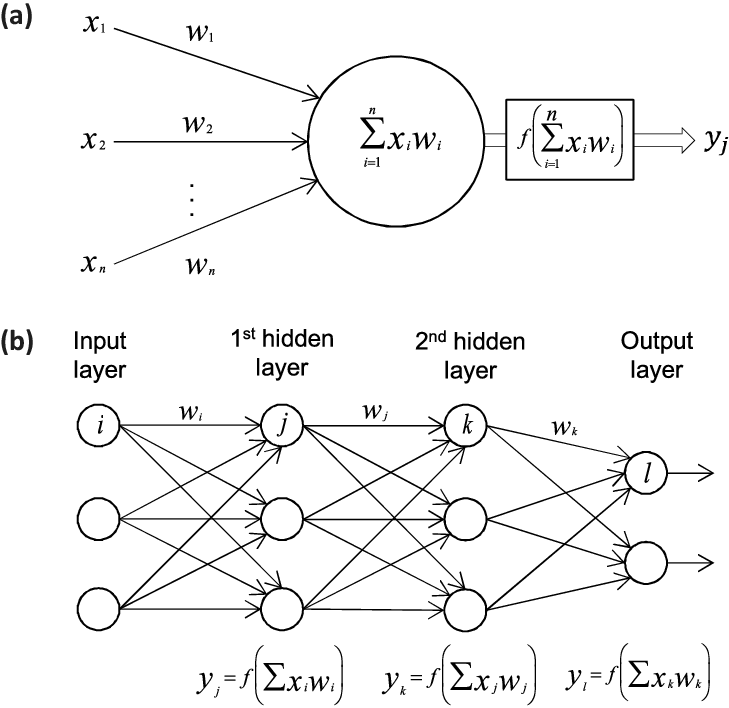
\includegraphics[width=0.8\linewidth]{figures/nns.png}}
  \caption{
  In a) we show a single perceptron model while in b) we dispay a network with two  hidden layers, an input layer and an output layer.
  }
\end{figure}
%\clearpage % flush figures
\end{frame}

\begin{frame}[plain,fragile]
\frametitle{Examples of XOR, OR and AND gates}

Let us first try to fit various gates using standard linear
regression. The gates we are thinking of are the classical XOR, OR and
AND gates, well-known elements in computer science. The tables here
show how we can set up the inputs $x_1$ and $x_2$ in order to yield a
specific target $y_i$.
































\begin{minted}[fontsize=\fontsize{9pt}{9pt},linenos=false,mathescape,baselinestretch=1.0,fontfamily=tt,xleftmargin=2mm]{python}
"""
Simple code that tests XOR, OR and AND gates with linear regression
"""

import numpy as np
# Design matrix
X = np.array([ [1, 0, 0], [1, 0, 1], [1, 1, 0],[1, 1, 1]],dtype=np.float64)
print(f"The X.TX  matrix:{X.T @ X}")
Xinv = np.linalg.pinv(X.T @ X)
print(f"The invers of X.TX  matrix:{Xinv}")

# The XOR gate 
yXOR = np.array( [ 0, 1 ,1, 0])
ThetaXOR  = Xinv @ X.T @ yXOR
print(f"The values of theta for the XOR gate:{ThetaXOR}")
print(f"The linear regression prediction  for the XOR gate:{X @ ThetaXOR}")


# The OR gate 
yOR = np.array( [ 0, 1 ,1, 1])
ThetaOR  = Xinv @ X.T @ yOR
print(f"The values of theta for the OR gate:{ThetaOR}")
print(f"The linear regression prediction  for the OR gate:{X @ ThetaOR}")


# The OR gate 
yAND = np.array( [ 0, 0 ,0, 1])
ThetaAND  = Xinv @ X.T @ yAND
print(f"The values of theta for the AND gate:{ThetaAND}")
print(f"The linear regression prediction  for the AND gate:{X @ ThetaAND}")

\end{minted}


What is happening here?
\end{frame}

\begin{frame}[plain,fragile]
\frametitle{Does Logistic Regression do a better Job?}

\begin{minted}[fontsize=\fontsize{9pt}{9pt},linenos=false,mathescape,baselinestretch=1.0,fontfamily=tt,xleftmargin=2mm]{python}
"""
Simple code that tests XOR and OR gates with linear regression
and logistic regression
"""

import matplotlib.pyplot as plt
from sklearn.linear_model import LogisticRegression
import numpy as np

# Design matrix
X = np.array([ [1, 0, 0], [1, 0, 1], [1, 1, 0],[1, 1, 1]],dtype=np.float64)
print(f"The X.TX  matrix:{X.T @ X}")
Xinv = np.linalg.pinv(X.T @ X)
print(f"The invers of X.TX  matrix:{Xinv}")

# The XOR gate 
yXOR = np.array( [ 0, 1 ,1, 0])
ThetaXOR  = Xinv @ X.T @ yXOR
print(f"The values of theta for the XOR gate:{ThetaXOR}")
print(f"The linear regression prediction  for the XOR gate:{X @ ThetaXOR}")


# The OR gate 
yOR = np.array( [ 0, 1 ,1, 1])
ThetaOR  = Xinv @ X.T @ yOR
print(f"The values of theta for the OR gate:{ThetaOR}")
print(f"The linear regression prediction  for the OR gate:{X @ ThetaOR}")


# The OR gate 
yAND = np.array( [ 0, 0 ,0, 1])
ThetaAND  = Xinv @ X.T @ yAND
print(f"The values of theta for the AND gate:{ThetaAND}")
print(f"The linear regression prediction  for the AND gate:{X @ ThetaAND}")

# Now we change to logistic regression


# Logistic Regression
logreg = LogisticRegression()
logreg.fit(X, yOR)
print("Test set accuracy with Logistic Regression for OR gate: {:.2f}".format(logreg.score(X,yOR)))

logreg.fit(X, yXOR)
print("Test set accuracy with Logistic Regression for XOR gate: {:.2f}".format(logreg.score(X,yXOR)))


logreg.fit(X, yAND)
print("Test set accuracy with Logistic Regression for AND gate: {:.2f}".format(logreg.score(X,yAND)))

\end{minted}


Not exactly impressive, but somewhat better.
\end{frame}

\begin{frame}[plain,fragile]
\frametitle{Adding Neural Networks}

\begin{minted}[fontsize=\fontsize{9pt}{9pt},linenos=false,mathescape,baselinestretch=1.0,fontfamily=tt,xleftmargin=2mm]{python}

# and now neural networks with Scikit-Learn and the XOR

from sklearn.neural_network import MLPClassifier
from sklearn.datasets import make_classification
X, yXOR = make_classification(n_samples=100, random_state=1)
FFNN = MLPClassifier(random_state=1, max_iter=300).fit(X, yXOR)
FFNN.predict_proba(X)
print(f"Test set accuracy with Feed Forward Neural Network  for XOR gate:{FFNN.score(X, yXOR)}")


\end{minted}
\end{frame}

\begin{frame}[plain,fragile]
\frametitle{Mathematics of deep learning}

\begin{block}{Two recent books online }
\begin{enumerate}
\item \href{{https://arxiv.org/abs/2105.04026}}{The Modern Mathematics of Deep Learning, by Julius Berner, Philipp Grohs, Gitta Kutyniok, Philipp Petersen}, published as \href{{https://doi.org/10.1017/9781009025096.002}}{Mathematical Aspects of Deep Learning, pp. 1-111. Cambridge University Press, 2022}

\item \href{{https://doi.org/10.48550/arXiv.2310.20360}}{Mathematical Introduction to Deep Learning: Methods, Implementations, and Theory, Arnulf Jentzen, Benno Kuckuck, Philippe von Wurstemberger}
\end{enumerate}

\noindent
\end{block}
\end{frame}

\begin{frame}[plain,fragile]
\frametitle{Reminder on books with hands-on material and codes}

\begin{block}{}
\begin{itemize}
\item \href{{https://sebastianraschka.com/blog/2022/ml-pytorch-book.html}}{Sebastian Rashcka et al, Machine learning with Sickit-Learn and PyTorch}
\end{itemize}

\noindent
\end{block}
\end{frame}

\begin{frame}[plain,fragile]
\frametitle{Reading recommendations}

\begin{enumerate}
\item Rashkca et al., chapter 11, jupyter-notebook sent separately, from \href{{https://github.com/rasbt/machine-learning-book}}{GitHub}

\item Goodfellow et al, chapter 6 and 7 contain most of the neural network background.
\end{enumerate}

\noindent
\end{frame}

\begin{frame}[plain,fragile]
\frametitle{Mathematics of deep learning and neural networks}

Neural networks, in its so-called feed-forward form, where each
iterations contains a feed-forward stage and a back-propgagation
stage, consist of series of affine matrix-matrix and matrix-vector
multiplications. The unknown parameters (the so-called biases and
weights which deternine the architecture of a neural network), are
uptaded iteratively using the so-called back-propagation algorithm.
This algorithm corresponds to the so-called reverse mode of 
automatic differentation.
\end{frame}

\begin{frame}[plain,fragile]
\frametitle{Basics of an NN}

A neural network consists of a series of hidden layers, in addition to
the input and output layers.  Each layer $l$ has a set of parameters
$\bm{\Theta}^{(l)}=(\bm{W}^{(l)},\bm{b}^{(l)})$ which are related to the
parameters in other layers through a series of affine transformations,
for a standard NN these are matrix-matrix and matrix-vector
multiplications.  For all layers we will simply use a collective variable $\bm{\Theta}$.

It consist of two basic steps:
\begin{enumerate}
\item a feed forward stage which takes a given input and produces a final output which is compared with the target values through our cost/loss function.

\item a back-propagation state where the unknown parameters $\bm{\Theta}$ are updated through the optimization of the their gradients. The expressions for the gradients are obtained via the chain rule, starting from the derivative of the cost/function.
\end{enumerate}

\noindent
These two steps make up one iteration. This iterative process is continued till we reach an eventual stopping criterion.
\end{frame}

\begin{frame}[plain,fragile]
\frametitle{Overarching view of a neural network}

The architecture of a neural network defines our model. This model
aims at describing some function $f(\bm{x}$ which represents
some final result (outputs or tagrget values) given a specific inpput
$\bm{x}$. Note that here $\bm{y}$ and $\bm{x}$ are not limited to be
vectors.

The architecture consists of
\begin{enumerate}
\item An input and an output layer where the input layer is defined by the inputs $\bm{x}$. The output layer produces the model ouput $\bm{\tilde{y}}$ which is compared with the target value $\bm{y}$

\item A given number of hidden layers and neurons/nodes/units for each layer (this may vary)

\item A given activation function $\sigma(\bm{z})$ with arguments $\bm{z}$ to be defined below. The activation functions may differ from layer to layer.

\item The last layer, normally called \textbf{output} layer has normally an activation function tailored to the specific problem

\item Finally we define a so-called cost or loss function which is used to gauge the quality of our model. 
\end{enumerate}

\noindent
\end{frame}

\begin{frame}[plain,fragile]
\frametitle{The optimization problem}

The cost function is a function of the unknown parameters
$\bm{\Theta}$ where the latter is a container for all possible
parameters needed to define a neural network

If we are dealing with a regression task a typical cost/loss function
is the mean squared error
\[
C(\bm{\Theta})=\frac{1}{n}\left\{\left(\bm{y}-\bm{X}\bm{\theta}\right)^T\left(\bm{y}-\bm{X}\bm{\theta}\right)\right\}.
\]
This function represents one of many possible ways to define
the so-called cost function. Note that here we have assumed a linear dependence in terms of the paramters $\bm{\Theta}$. This is in general not the case.
\end{frame}

\begin{frame}[plain,fragile]
\frametitle{Parameters of neural networks}

For neural networks the parameters
$\bm{\Theta}$ are given by the so-called weights and biases (to be
defined below).

The weights are given by matrix elements $w_{ij}^{(l)}$ where the
superscript indicates the layer number. The biases are typically given
by vector elements representing each single node of a given layer,
that is $b_j^{(l)}$.
\end{frame}

\begin{frame}[plain,fragile]
\frametitle{Other ingredients of a neural network}

Having defined the architecture of a neural network, the optimization
of the cost function with respect to the parameters $\bm{\Theta}$,
involves the calculations of gradients and their optimization. The
gradients represent the derivatives of a multidimensional object and
are often approximated by various gradient methods, including
\begin{enumerate}
\item various quasi-Newton methods,

\item plain gradient descent (GD) with a constant learning rate $\eta$,

\item GD with momentum and other approximations to the learning rates such as
\begin{itemize}

  \item Adapative gradient (ADAgrad)

  \item Root mean-square propagation (RMSprop)

  \item Adaptive gradient with momentum (ADAM) and many other

\end{itemize}

\noindent
\item Stochastic gradient descent and various families of learning rate approximations
\end{enumerate}

\noindent
\end{frame}

\begin{frame}[plain,fragile]
\frametitle{Other parameters}

In addition to the above, there are often additional hyperparamaters
which are included in the setup of a neural network. These will be
discussed below.
\end{frame}

\begin{frame}[plain,fragile]
\frametitle{Universal approximation theorem}

The universal approximation theorem plays a central role in deep
learning.  \href{{https://link.springer.com/article/10.1007/BF02551274}}{Cybenko (1989)} showed
the following:

\begin{block}{}
Let $\sigma$ be any continuous sigmoidal function such that
\[
\sigma(z) = \left\{\begin{array}{cc} 1 & z\rightarrow \infty\\ 0 & z \rightarrow -\infty \end{array}\right.
\]
Given a continuous and deterministic function $F(\bm{x})$ on the unit
cube in $d$-dimensions $F\in [0,1]^d$, $x\in [0,1]^d$ and a parameter
$\epsilon >0$, there is a one-layer (hidden) neural network
$f(\bm{x};\bm{\Theta})$ with $\bm{\Theta}=(\bm{W},\bm{b})$ and $\bm{W}\in
\mathbb{R}^{m\times n}$ and $\bm{b}\in \mathbb{R}^{n}$, for which
\[
\vert F(\bm{x})-f(\bm{x};\bm{\Theta})\vert < \epsilon \hspace{0.1cm} \forall \bm{x}\in[0,1]^d.
\]

\end{block}
\end{frame}

\begin{frame}[plain,fragile]
\frametitle{Some parallels from real analysis}

For those of you familiar with for example the \href{{https://en.wikipedia.org/wiki/Stone%E2%80%93Weierstrass_theorem}}{Stone-Weierstrass
theorem}
for polynomial approximations or the convergence criterion for Fourier
series, there are similarities in the derivation of the proof for
neural networks.
\end{frame}

\begin{frame}[plain,fragile]
\frametitle{The approximation theorem in words}

\textbf{Any continuous function $y=F(\bm{x})$ supported on the unit cube in
$d$-dimensions can be approximated by a one-layer sigmoidal network to
arbitrary accuracy.}

\href{{https://www.sciencedirect.com/science/article/abs/pii/089360809190009T}}{Hornik (1991)} extended the theorem by letting any non-constant, bounded activation function to be included using that the expectation value
\[
\mathbb{E}[\vert F(\bm{x})\vert^2] =\int_{\bm{x}\in D} \vert F(\bm{x})\vert^2p(\bm{x})d\bm{x} < \infty.
\]
Then we have
\[
\mathbb{E}[\vert F(\bm{x})-f(\bm{x};\bm{\Theta})\vert^2] =\int_{\bm{x}\in D} \vert F(\bm{x})-f(\bm{x};\bm{\Theta})\vert^2p(\bm{x})d\bm{x} < \epsilon.
\]
\end{frame}

\begin{frame}[plain,fragile]
\frametitle{More on the general approximation theorem}

None of the proofs give any insight into the relation between the
number of of hidden layers and nodes and the approximation error
$\epsilon$, nor the magnitudes of $\bm{W}$ and $\bm{b}$.

Neural networks (NNs) have what we may call a kind of universality no matter what function we want to compute.

\begin{block}{}
It does not mean that an NN can be used to exactly compute any function. Rather, we get an approximation that is as good as we want. 
\end{block}
\end{frame}

\begin{frame}[plain,fragile]
\frametitle{Class of functions we can approximate}

\begin{block}{}
The class of functions that can be approximated are the continuous ones.
If the function $F(\bm{x})$ is discontinuous, it won't in general be possible to approximate it. However, an NN may still give an approximation even if we fail in some points.
\end{block}
\end{frame}

\begin{frame}[plain,fragile]
\frametitle{Setting up the equations for a neural network}

The questions we want to ask are how do changes in the biases and the
weights in our network change the cost function and how can we use the
final output to modify the weights and biases?

To derive these equations let us start with a plain regression problem
and define our cost function as

\[
{\cal C}(\bm{\Theta})  =  \frac{1}{2}\sum_{i=1}^n\left(y_i - \tilde{y}_i\right)^2, 
\]

where the $y_i$s are our $n$ targets (the values we want to
reproduce), while the outputs of the network after having propagated
all inputs $\bm{x}$ are given by $\bm{\tilde{y}}_i$.
\end{frame}

\begin{frame}[plain,fragile]
\frametitle{Layout of a neural network with three hidden layers}

\vspace{6mm}

% inline figure
\centerline{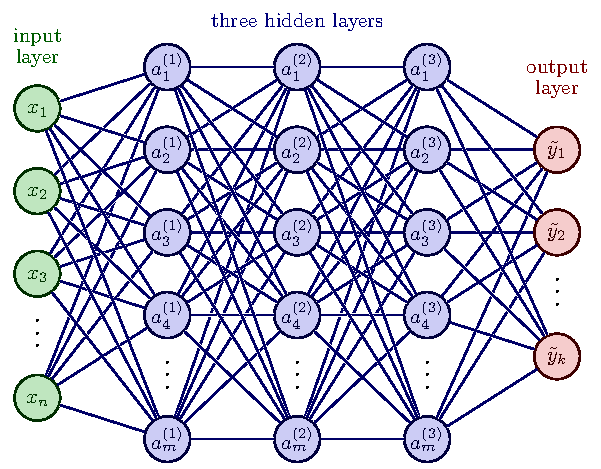
\includegraphics[width=1.0\linewidth]{figures/nn1.pdf}}

\vspace{6mm}
\end{frame}

\begin{frame}[plain,fragile]
\frametitle{Definitions}

With our definition of the targets $\bm{y}$, the outputs of the
network $\bm{\tilde{y}}$ and the inputs $\bm{x}$ we
define now the activation $z_j^l$ of node/neuron/unit $j$ of the
$l$-th layer as a function of the bias, the weights which add up from
the previous layer $l-1$ and the forward passes/outputs
$\hat{a}^{l-1}$ from the previous layer as

\[
z_j^l = \sum_{i=1}^{M_{l-1}}w_{ij}^la_i^{l-1}+b_j^l,
\]

where $b_k^l$ are the biases from layer $l$.  Here $M_{l-1}$
represents the total number of nodes/neurons/units of layer $l-1$. The
figure in the whiteboard notes illustrates this equation.  We can rewrite this in a more
compact form as the matrix-vector products we discussed earlier,

\[
\hat{z}^l = \left(\hat{W}^l\right)^T\hat{a}^{l-1}+\hat{b}^l.
\]
\end{frame}

\begin{frame}[plain,fragile]
\frametitle{Inputs to the activation function}

With the activation values $\bm{z}^l$ we can in turn define the
output of layer $l$ as $\bm{a}^l = f(\bm{z}^l)$ where $f$ is our
activation function. In the examples here we will use the sigmoid
function discussed in our logistic regression lectures. We will also use the same activation function $f$ for all layers
and their nodes.  It means we have

\[
a_j^l = \sigma(z_j^l) = \frac{1}{1+\exp{-(z_j^l)}}.
\]
\end{frame}

\begin{frame}[plain,fragile]
\frametitle{Derivatives and the chain rule}

From the definition of the activation $z_j^l$ we have
\[
\frac{\partial z_j^l}{\partial w_{ij}^l} = a_i^{l-1},
\]
and
\[
\frac{\partial z_j^l}{\partial a_i^{l-1}} = w_{ji}^l. 
\]

With our definition of the activation function we have that (note that this function depends only on $z_j^l$)
\[
\frac{\partial a_j^l}{\partial z_j^{l}} = a_j^l(1-a_j^l)=\sigma(z_j^l)(1-\sigma(z_j^l)). 
\]
\end{frame}

\begin{frame}[plain,fragile]
\frametitle{Derivative of the cost function}

With these definitions we can now compute the derivative of the cost function in terms of the weights.

Let us specialize to the output layer $l=L$. Our cost function is
\[
{\cal C}(\bm{\Theta}^L)  =  \frac{1}{2}\sum_{i=1}^n\left(y_i - \tilde{y}_i\right)^2=\frac{1}{2}\sum_{i=1}^n\left(a_i^L - y_i\right)^2, 
\]
The derivative of this function with respect to the weights is

\[
\frac{\partial{\cal C}(\bm{\Theta}^L)}{\partial w_{jk}^L}  =  \left(a_j^L - y_j\right)\frac{\partial a_j^L}{\partial w_{jk}^{L}}, 
\]
The last partial derivative can easily be computed and reads (by applying the chain rule)
\[
\frac{\partial a_j^L}{\partial w_{jk}^{L}} = \frac{\partial a_j^L}{\partial z_{j}^{L}}\frac{\partial z_j^L}{\partial w_{jk}^{L}}=a_j^L(1-a_j^L)a_k^{L-1}.  
\]
\end{frame}

\begin{frame}[plain,fragile]
\frametitle{Simpler examples first, and automatic differentiation}

In order to understand the back propagation algorithm and its
derivation (an implementation of the chain rule), let us first digress
with some simple examples. These examples are also meant to motivate
the link with back propagation and \href{{https://en.wikipedia.org/wiki/Automatic_differentiation}}{automatic differentiation}.
\end{frame}

\begin{frame}[plain,fragile]
\frametitle{Reminder on the chain rule and gradients}

If we have a multivariate function $f(x,y)$ where $x=x(t)$ and $y=y(t)$ are functions of a variable $t$, we have that the gradient of $f$ with respect to $t$ (without the explicit unit vector components)
\[
\frac{df}{dt} = \begin{bmatrix}\frac{\partial f}{\partial x} & \frac{\partial f}{\partial y} \end{bmatrix} \begin{bmatrix}\frac{\partial x}{\partial t} \\ \frac{\partial y}{\partial t} \end{bmatrix}=\frac{\partial f}{\partial x} \frac{\partial x}{\partial t} +\frac{\partial f}{\partial y} \frac{\partial y}{\partial t}. 
\]
\end{frame}

\begin{frame}[plain,fragile]
\frametitle{Multivariable functions}

If we have a multivariate function $f(x,y)$ where $x=x(t,s)$ and $y=y(t,s)$ are functions of the variables $t$ and $s$, we have that the partial derivatives
\[
\frac{\partial f}{\partial s}=\frac{\partial f}{\partial x}\frac{\partial x}{\partial s}+\frac{\partial f}{\partial y}\frac{\partial y}{\partial s},
\]
and
\[
\frac{\partial f}{\partial t}=\frac{\partial f}{\partial x}\frac{\partial x}{\partial t}+\frac{\partial f}{\partial y}\frac{\partial y}{\partial t}.
\]

the gradient of $f$ with respect to $t$ and $s$ (without the explicit unit vector components)
\[
\frac{df}{d(s,t)} = \begin{bmatrix}\frac{\partial f}{\partial x} & \frac{\partial f}{\partial y} \end{bmatrix} \begin{bmatrix}\frac{\partial x}{\partial s}  &\frac{\partial x}{\partial t} \\ \frac{\partial y}{\partial s} & \frac{\partial y}{\partial t} \end{bmatrix}.
\]
\end{frame}

\begin{frame}[plain,fragile]
\frametitle{Automatic differentiation through examples}

A great introduction to automatic differentiation is given by Baydin et al., see \href{{https://arxiv.org/abs/1502.05767}}{\nolinkurl{https://arxiv.org/abs/1502.05767}}.

Automatic differentiation is a represented by a repeated application
of the chain rule on well-known functions and allows for the
calculation of derivatives to numerical precision. It is not the same
as the calculation of symbolic derivatives via for example SymPy, nor
does it use approximative formulae based on Taylor-expansions of a
function around a given value. The latter are error prone due to
truncation errors and values of the step size $\Delta$.
\end{frame}

\begin{frame}[plain,fragile]
\frametitle{Simple example}

Our first example is rather simple,
\[
f(x) =\exp{x^2},
\]
with derivative
\[
f'(x) =2x\exp{x^2}.
\]
We can use SymPy to extract the pertinent lines of Python code through the following simple example









\begin{minted}[fontsize=\fontsize{9pt}{9pt},linenos=false,mathescape,baselinestretch=1.0,fontfamily=tt,xleftmargin=2mm]{python}
from __future__ import division
from sympy import *
x = symbols('x')
expr = exp(x*x)
simplify(expr)
derivative = diff(expr,x)
print(python(expr))
print(python(derivative))

\end{minted}
\end{frame}

\begin{frame}[plain,fragile]
\frametitle{Smarter way of evaluating the above function}

If we study this function, we note that we can reduce the number of operations by introducing an intermediate variable
\[
a = x^2,
\]
leading to 
\[
f(x) = f(a(x)) = b= \exp{a}.
\]

We now assume that all operations can be counted in terms of equal
floating point operations. This means that in order to calculate
$f(x)$ we need first to square $x$ and then compute the exponential. We
have thus two floating point operations only.
\end{frame}

\begin{frame}[plain,fragile]
\frametitle{Reducing the number of operations}

With the introduction of a precalculated quantity $a$ and thereby $f(x)$ we have that the derivative can be written as

\[
f'(x) = 2xb,
\]

which reduces the number of operations from four in the orginal
expression to two. This means that if we need to compute $f(x)$ and
its derivative (a common task in optimizations), we have reduced the
number of operations from six to four in total.

\textbf{Note} that the usage of a symbolic software like SymPy does not
include such simplifications and the calculations of the function and
the derivatives yield in general more floating point operations.
\end{frame}

\begin{frame}[plain,fragile]
\frametitle{Chain rule, forward and reverse modes}

In the above example we have introduced the variables $a$ and $b$, and our function is
\[
f(x) = f(a(x)) = b= \exp{a},
\]
with $a=x^2$. We can decompose the derivative of $f$ with respect to $x$ as
\[
\frac{df}{dx}=\frac{df}{db}\frac{db}{da}\frac{da}{dx}.
\]

We note that since $b=f(x)$ that
\[
\frac{df}{db}=1,
\]
leading to
\[
\frac{df}{dx}=\frac{db}{da}\frac{da}{dx}=2x\exp{x^2},
\]
as before.
\end{frame}

\begin{frame}[plain,fragile]
\frametitle{Forward and reverse modes}

We have that 
\[
\frac{df}{dx}=\frac{df}{db}\frac{db}{da}\frac{da}{dx},
\]
which we can rewrite either as
\[
\frac{df}{dx}=\left[\frac{df}{db}\frac{db}{da}\right]\frac{da}{dx},
\]
or
\[
\frac{df}{dx}=\frac{df}{db}\left[\frac{db}{da}\frac{da}{dx}\right].
\]

The first expression is called reverse mode (or back propagation)
since we start by evaluating the derivatives at the end point and then
propagate backwards. This is the standard way of evaluating
derivatives (gradients) when optimizing the parameters of a neural
network.  In the context of deep learning this is computationally
more efficient since the output of a neural network consists of either
one or some few other output variables.

The second equation defines the so-called  \textbf{forward mode}.
\end{frame}

\begin{frame}[plain,fragile]
\frametitle{More complicated function}

We increase our ambitions and introduce a slightly more complicated function
\[
f(x) =\sqrt{x^2+exp{x^2}},
\]
with derivative
\[
f'(x) =\frac{x(1+\exp{x^2})}{\sqrt{x^2+exp{x^2}}}.
\]
The corresponding SymPy code reads









\begin{minted}[fontsize=\fontsize{9pt}{9pt},linenos=false,mathescape,baselinestretch=1.0,fontfamily=tt,xleftmargin=2mm]{python}
from __future__ import division
from sympy import *
x = symbols('x')
expr = sqrt(x*x+exp(x*x))
simplify(expr)
derivative = diff(expr,x)
print(python(expr))
print(python(derivative))

\end{minted}
\end{frame}

\begin{frame}[plain,fragile]
\frametitle{Counting the number of floating point operations}

A simple count of operations shows that we need five operations for
the function itself and ten for the derivative.  Fifteen operations in total if we wish to proceed with the above codes.

Can we reduce this to
say half the number of operations?
\end{frame}

\begin{frame}[plain,fragile]
\frametitle{Defining intermediate operations}

We can indeed reduce the number of operation to half of those listed in the brute force approach above.
We define the following quantities
\[
a = x^2,
\]
and
\[
b = \exp{x^2} = \exp{a},
\]
and
\[
c= a+b,
\]
and
\[
d=f(x)=\sqrt{c}.
\]
\end{frame}

\begin{frame}[plain,fragile]
\frametitle{New expression for the derivative}

With these definitions we obtain the following partial derivatives 
\[
\frac{\partial a}{\partial x} = 2x,
\]
and
\[
\frac{\partial b}{\partial a} = \exp{a},
\]
and
\[
\frac{\partial c}{\partial a} = 1,
\]
and
\[
\frac{\partial c}{\partial b} = 1,
\]
and
\[
\frac{\partial d}{\partial c} = \frac{1}{2\sqrt{c}},
\]
and finally
\[
\frac{\partial f}{\partial d} = 1.
\]
\end{frame}

\begin{frame}[plain,fragile]
\frametitle{Final derivatives}

Our final derivatives are thus
\[
\frac{\partial f}{\partial c} = \frac{\partial f}{\partial d} \frac{\partial d}{\partial c}  = \frac{1}{2\sqrt{c}},
\]
\[
\frac{\partial f}{\partial b} = \frac{\partial f}{\partial c} \frac{\partial c}{\partial b}  = \frac{1}{2\sqrt{c}},
\]
\[
\frac{\partial f}{\partial a} = \frac{\partial f}{\partial c} \frac{\partial c}{\partial a}+
\frac{\partial f}{\partial b} \frac{\partial b}{\partial a}  = \frac{1+\exp{a}}{2\sqrt{c}},
\]
and finally 
\[
\frac{\partial f}{\partial x} = \frac{\partial f}{\partial a} \frac{\partial a}{\partial x}  = \frac{x(1+\exp{a})}{\sqrt{c}},
\]
which is just
\[
\frac{\partial f}{\partial x} = \frac{x(1+b)}{d},
\]
and requires only three operations if we can reuse all intermediate variables.
\end{frame}

\begin{frame}[plain,fragile]
\frametitle{In general not this simple}

In general, see the generalization below, unless we can obtain simple
analytical expressions which we can simplify further, the final
implementation of automatic differentiation involves repeated
calculations (and thereby operations) of derivatives of elementary
functions.
\end{frame}

\begin{frame}[plain,fragile]
\frametitle{Automatic differentiation}

We can make this example more formal. Automatic differentiation is a
formalization of the previous example (see graph).

We define $\bm{x}\in x_1,\dots, x_l$ input variables to a given function $f(\bm{x})$ and $x_{l+1},\dots, x_L$ intermediate variables.

In the above example we have only one input variable, $l=1$ and four intermediate variables, that is
\[
\begin{bmatrix} x_1=x & x_2 = x^2=a & x_3 =\exp{a}= b & x_4=c=a+b & x_5 = \sqrt{c}=d \end{bmatrix}.
\]

Furthemore, for $i=l+1, \dots, L$ (here $i=2,3,4,5$ and $f=x_L=d$), we
define the elementary functions $g_i(x_{Pa(x_i)})$ where $x_{Pa(x_i)}$ are the parent nodes of the variable $x_i$.

In our case, we have for example for $x_3=g_3(x_{Pa(x_i)})=\exp{a}$, that $g_3=\exp{()}$ and $x_{Pa(x_3)}=a$.
\end{frame}

\begin{frame}[plain,fragile]
\frametitle{Chain rule}

We can now compute the gradients by back-propagating the derivatives using the chain rule.
We have defined
\[
\frac{\partial f}{\partial x_L} = 1,
\]
which allows us to find the derivatives of the various variables $x_i$ as
\[
\frac{\partial f}{\partial x_i} = \sum_{x_j:x_i\in Pa(x_j)}\frac{\partial f}{\partial x_j} \frac{\partial x_j}{\partial x_i}=\sum_{x_j:x_i\in Pa(x_j)}\frac{\partial f}{\partial x_j} \frac{\partial g_j}{\partial x_i}.
\]

Whenever we have a function which can be expressed as a computation
graph and the various functions can be expressed in terms of
elementary functions that are differentiable, then automatic
differentiation works.  The functions may not need to be elementary
functions, they could also be computer programs, although not all
programs can be automatically differentiated.
\end{frame}

\begin{frame}[plain,fragile]
\frametitle{First network example, simple percepetron with one input}

As yet another example we define now a simple perceptron model with
all quantities given by scalars. We consider only one input variable
$x$ and one target value $y$.  We define an activation function
$\sigma_1$ which takes as input

\[
z_1 = w_1x+b_1,
\]
where $w_1$ is the weight and $b_1$ is the bias. These are the
parameters we want to optimize.  The output is $a_1=\sigma(z_1)$ (see
graph from whiteboard notes). This output is then fed into the
\textbf{cost/loss} function, which we here for the sake of simplicity just
define as the squared error

\[
C(x;w_1,b_1)=\frac{1}{2}(a_1-y)^2.
\]
\end{frame}

\begin{frame}[plain,fragile]
\frametitle{Layout of a simple neural network with no hidden layer}

\vspace{6mm}

% inline figure
\centerline{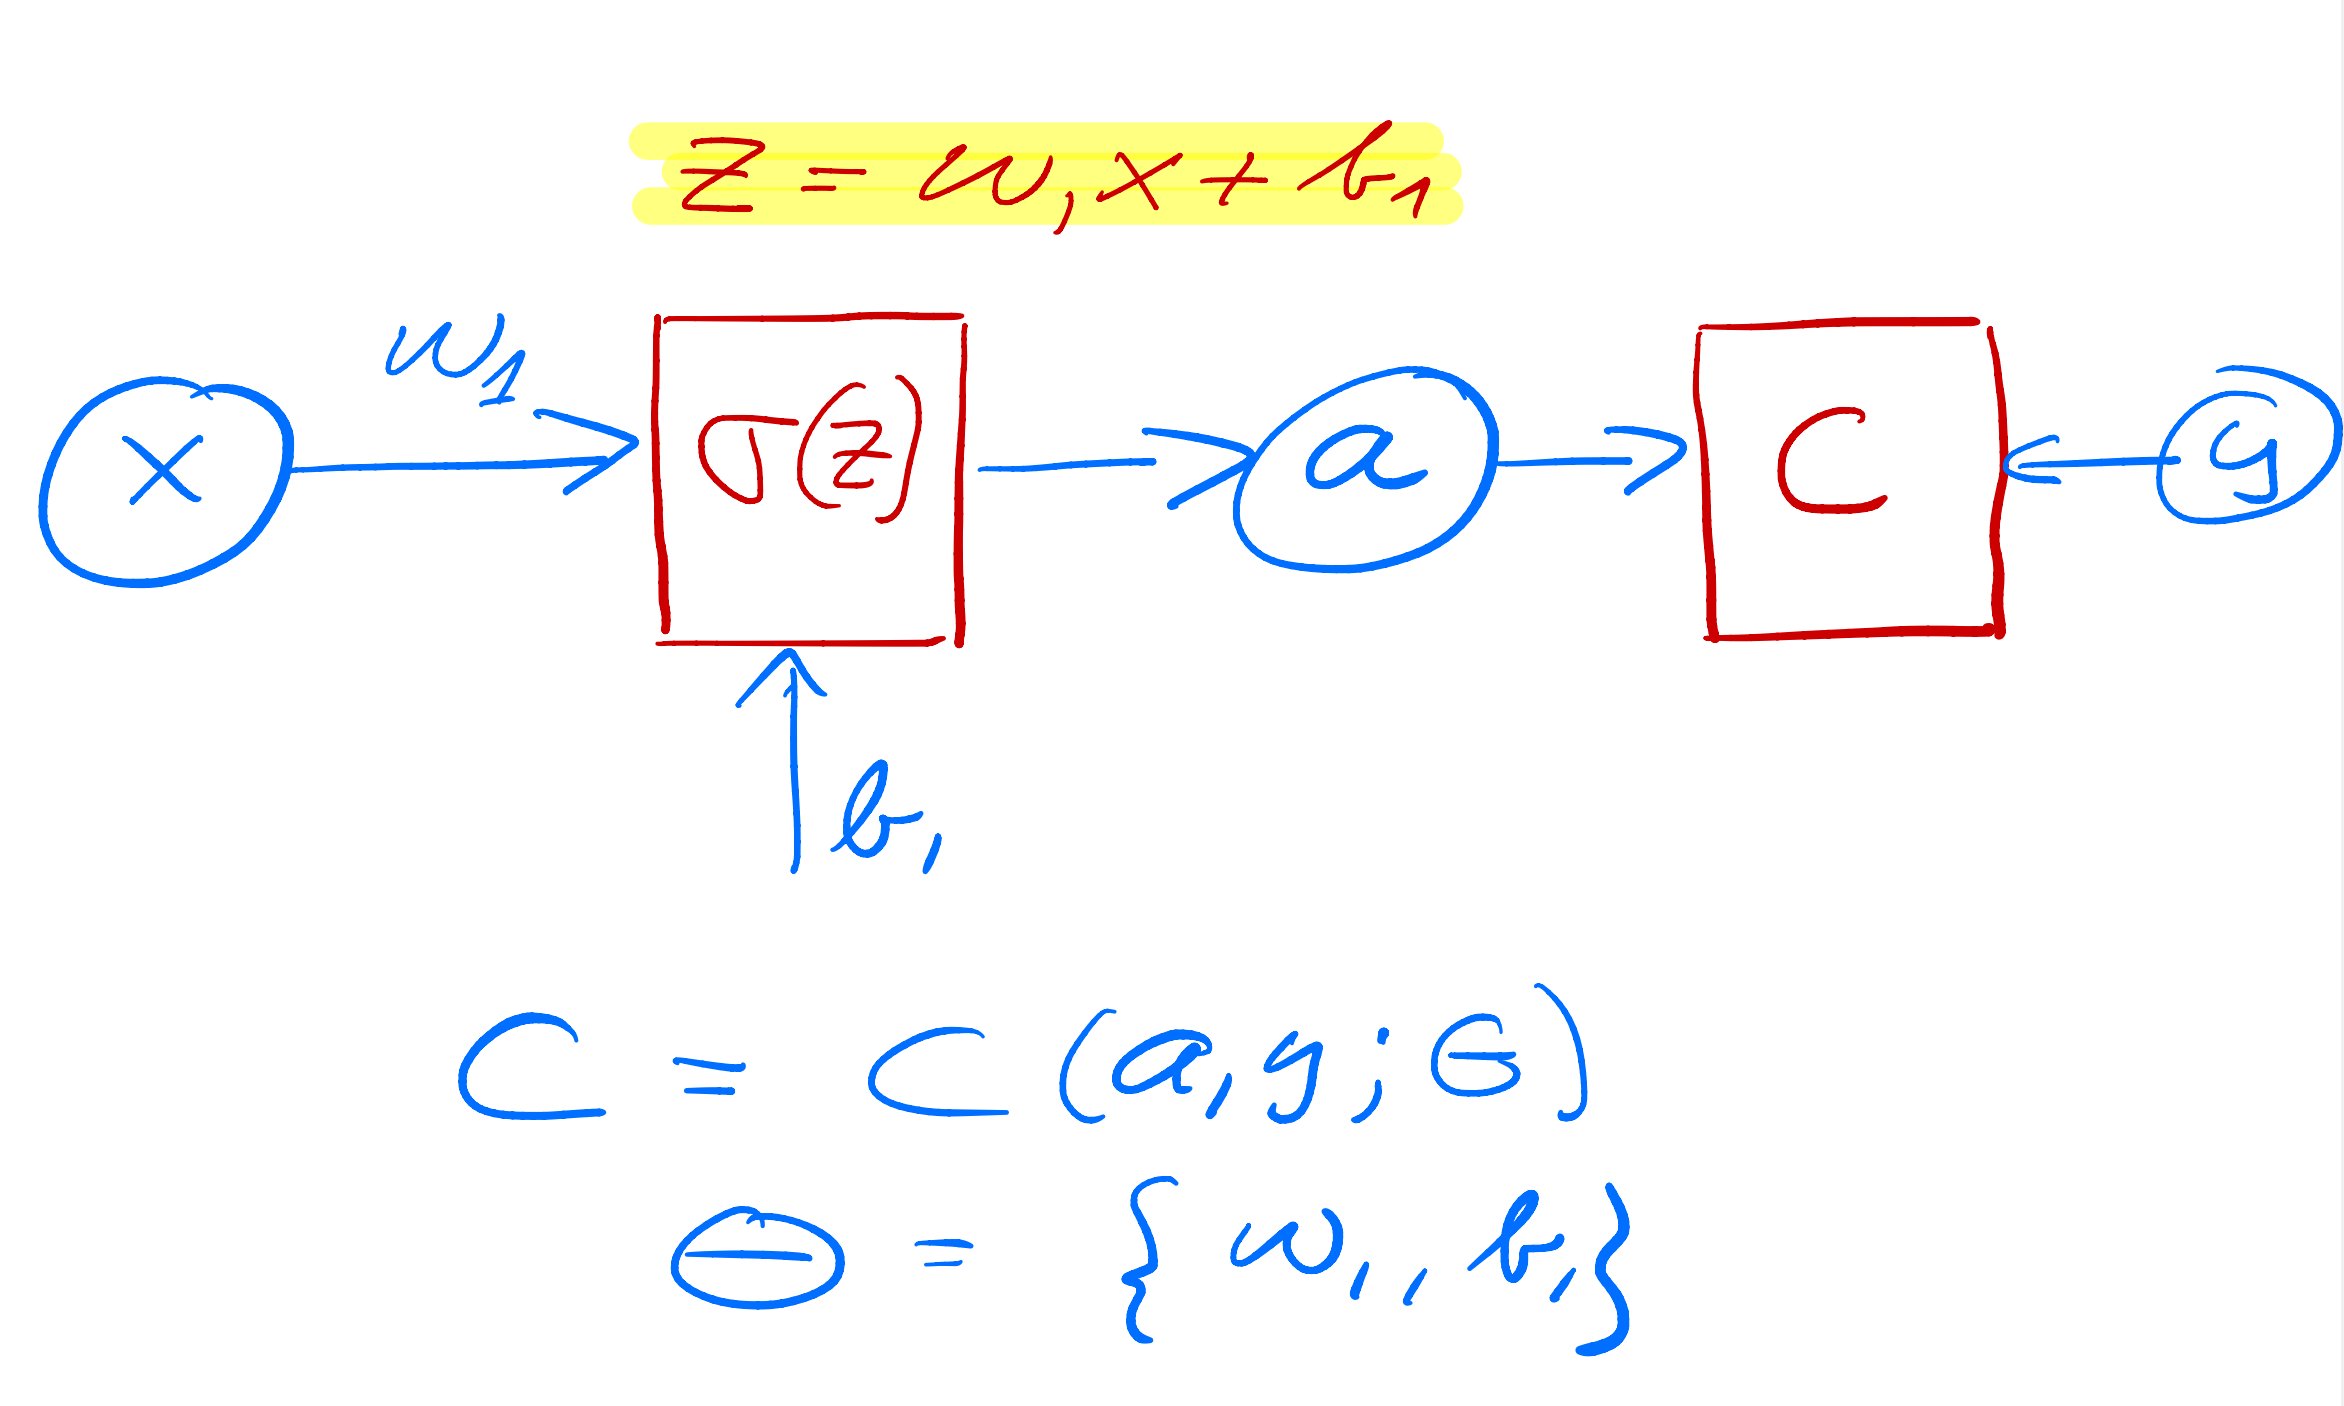
\includegraphics[width=1.0\linewidth]{figures/simplenn1.png}}

\vspace{6mm}
\end{frame}

\begin{frame}[plain,fragile]
\frametitle{Optimizing the parameters}

In setting up the feed forward and back propagation parts of the
algorithm, we need now the derivative of the various variables we want
to train.

We need
\[
\frac{\partial C}{\partial w_1} \hspace{0.1cm}\mathrm{and}\hspace{0.1cm}\frac{\partial C}{\partial b_1}. 
\]

Using the chain rule we find 
\[
\frac{\partial C}{\partial w_1}=\frac{\partial C}{\partial a_1}\frac{\partial a_1}{\partial z_1}\frac{\partial z_1}{\partial w_1}=(a_1-y)\sigma_1'x,
\]
and
\[
\frac{\partial C}{\partial b_1}=\frac{\partial C}{\partial a_1}\frac{\partial a_1}{\partial z_1}\frac{\partial z_1}{\partial b_1}=(a_1-y)\sigma_1',
\]
which we later will just define as
\[
\frac{\partial C}{\partial a_1}\frac{\partial a_1}{\partial z_1}=\delta_1.
\]
\end{frame}

\begin{frame}[plain,fragile]
\frametitle{Adding a hidden layer}

We change our simple model to (see graph)
a network with just one hidden layer but with scalar variables only.

Our output variable changes to $a_2$ and $a_1$ is now the output from the hidden node and $a_0=x$.
We have then
\[
z_1 = w_1a_0+b_1 \hspace{0.1cm} \wedge a_1 = \sigma_1(z_1),
\]
\[
z_2 = w_2a_1+b_2 \hspace{0.1cm} \wedge a_2 = \sigma_2(z_2),
\]
and the cost function
\[
C(x;\bm{\Theta})=\frac{1}{2}(a_2-y)^2,
\]
with $\bm{\Theta}=[w_1,w_2,b_1,b_2]$.
\end{frame}

\begin{frame}[plain,fragile]
\frametitle{Layout of a simple neural network with one hidden layer}

\vspace{6mm}

% inline figure
\centerline{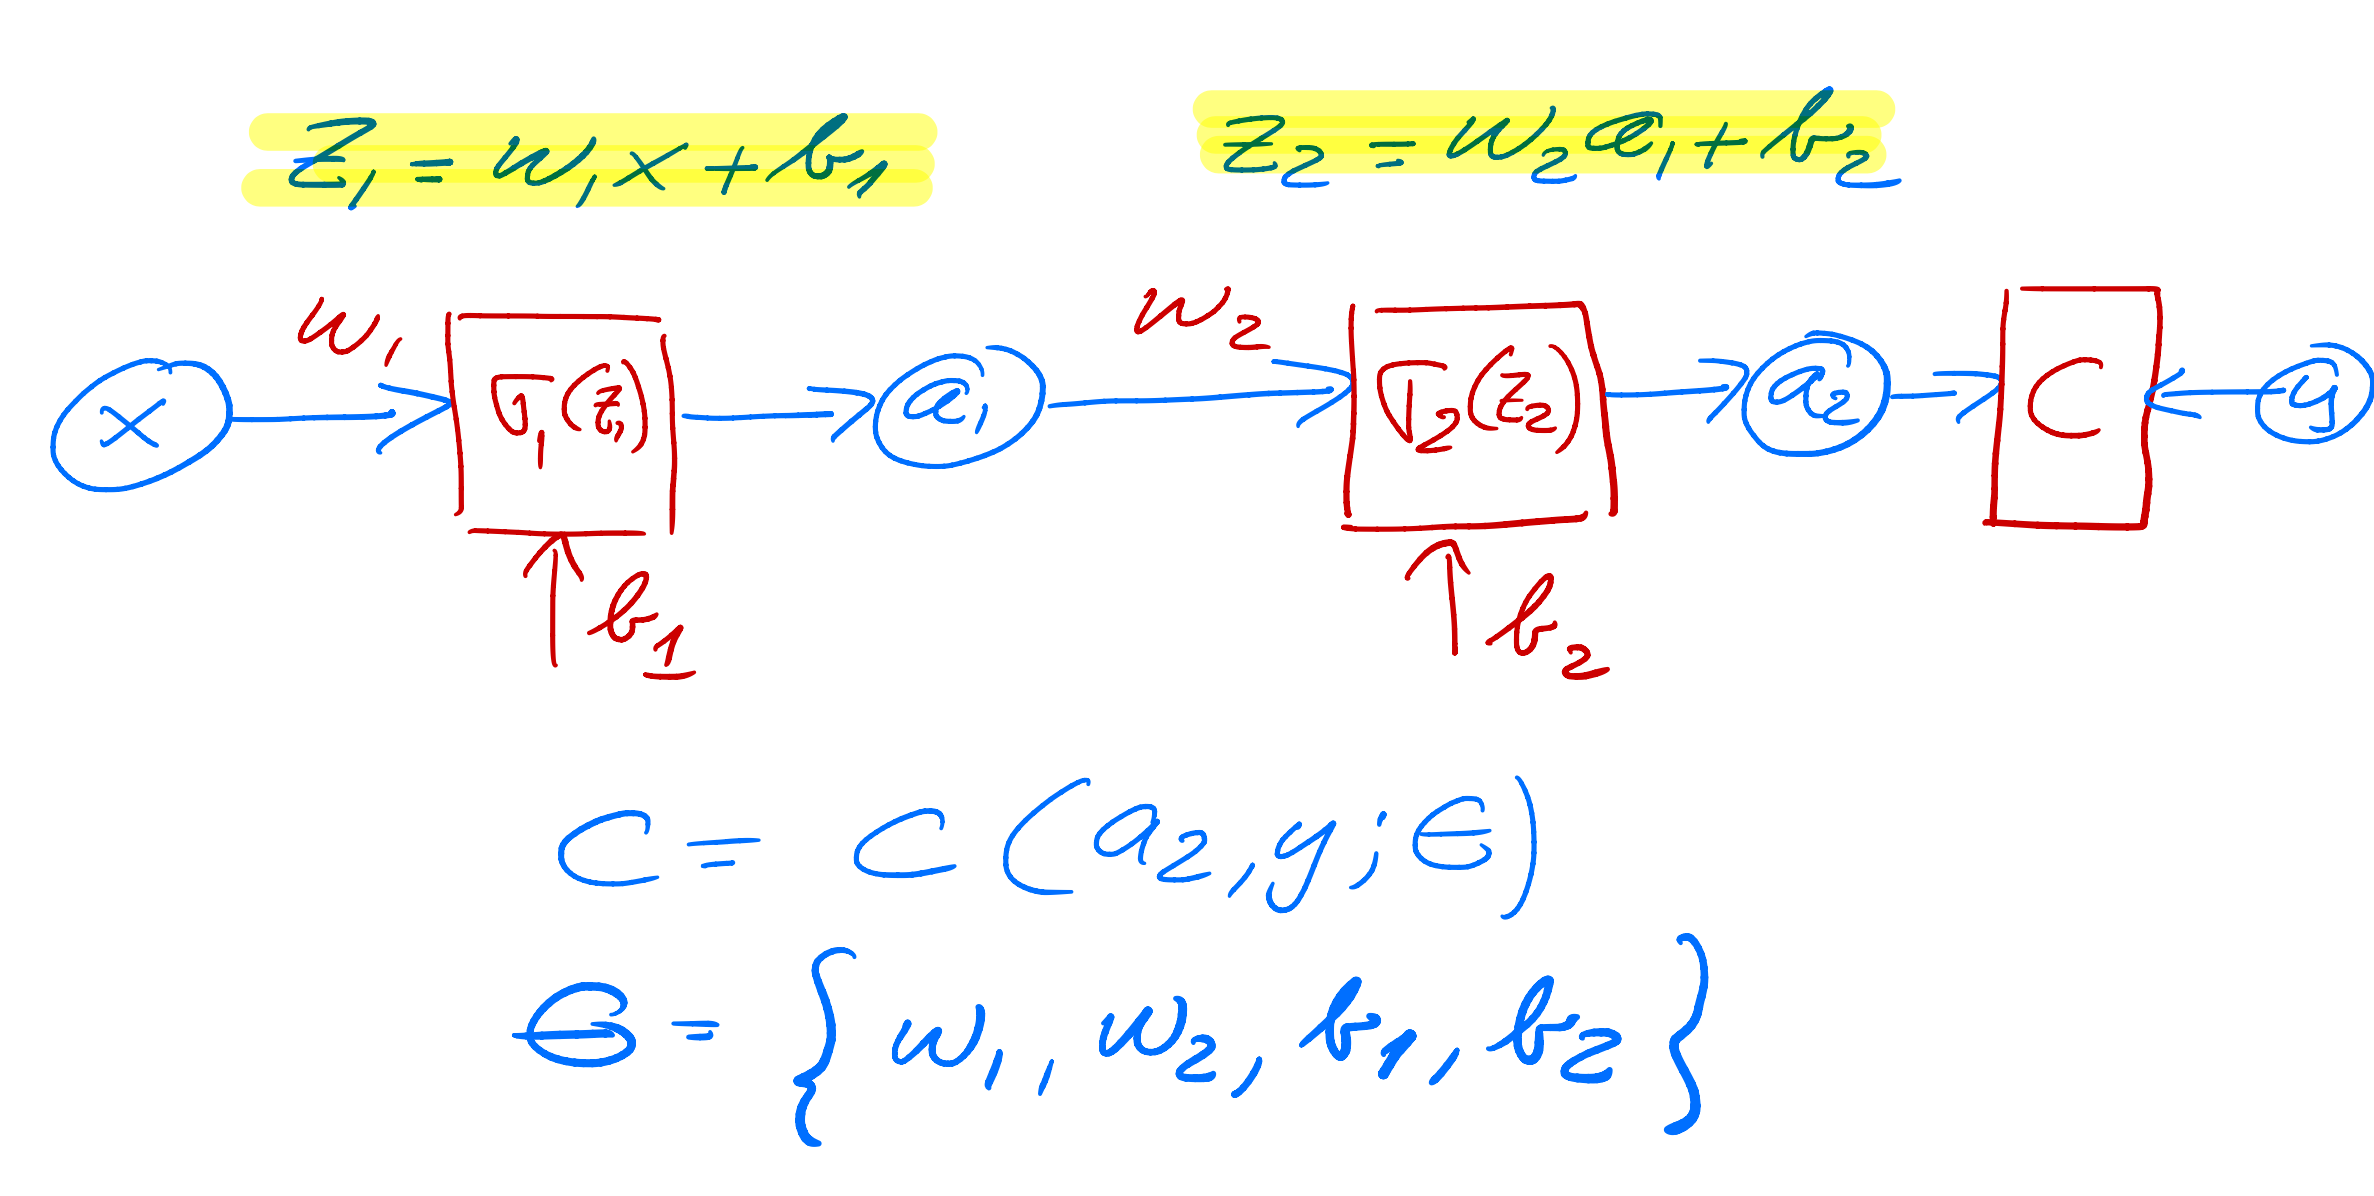
\includegraphics[width=1.0\linewidth]{figures/simplenn2.png}}

\vspace{6mm}
\end{frame}

\begin{frame}[plain,fragile]
\frametitle{The derivatives}

The derivatives are now, using the chain rule again

\[
\frac{\partial C}{\partial w_2}=\frac{\partial C}{\partial a_2}\frac{\partial a_2}{\partial z_2}\frac{\partial z_2}{\partial w_2}=(a_2-y)\sigma_2'a_1=\delta_2a_1,
\]
\[
\frac{\partial C}{\partial b_2}=\frac{\partial C}{\partial a_2}\frac{\partial a_2}{\partial z_2}\frac{\partial z_2}{\partial b_2}=(a_2-y)\sigma_2'=\delta_2,
\]
\[
\frac{\partial C}{\partial w_1}=\frac{\partial C}{\partial a_2}\frac{\partial a_2}{\partial z_2}\frac{\partial z_2}{\partial a_1}\frac{\partial a_1}{\partial z_1}\frac{\partial z_1}{\partial w_1}=(a_2-y)\sigma_2'a_1\sigma_1'a_0,
\]
\[
\frac{\partial C}{\partial b_1}=\frac{\partial C}{\partial a_2}\frac{\partial a_2}{\partial z_2}\frac{\partial z_2}{\partial a_1}\frac{\partial a_1}{\partial z_1}\frac{\partial z_1}{\partial b_1}=(a_2-y)\sigma_2'\sigma_1'=\delta_1.
\]

Can you generalize this to more than one hidden layer?
\end{frame}

\begin{frame}[plain,fragile]
\frametitle{Important observations}

\begin{block}{}
From the above equations we see that the derivatives of the activation
functions play a central role. If they vanish, the training may
stop. This is called the vanishing gradient problem, see discussions below. If they become
large, the parameters $w_i$ and $b_i$ may simply go to infinity. This
is referenced as  the exploding gradient problem.
\end{block}
\end{frame}

\begin{frame}[plain,fragile]
\frametitle{The training}

The training of the parameters is done through various gradient descent approximations with

\[
w_{i}\leftarrow w_{i}- \eta \delta_i a_{i-1},
\]
and
\[
b_i \leftarrow b_i-\eta \delta_i,
\]
with $\eta$ is the learning rate.

One iteration consists of one feed forward step and one back-propagation step. Each back-propagation step does one update of the parameters $\bm{\Theta}$.

For the first hidden layer $a_{i-1}=a_0=x$ for this simple model.
\end{frame}

\begin{frame}[plain,fragile]
\frametitle{Code example}

The code here implements the above model with one hidden layer and
scalar variables for the same function we studied in the previous
example.  The code is however set up so that we can add multiple
inputs $x$ and target values $y$. Note also that we have the
possibility of defining a feature matrix $\bm{X}$ with more than just
one column for the input values. This will turn useful in our next example. We have also defined matrices and vectors for all of our operations although it is not necessary here.


































































\begin{minted}[fontsize=\fontsize{9pt}{9pt},linenos=false,mathescape,baselinestretch=1.0,fontfamily=tt,xleftmargin=2mm]{python}
import numpy as np
# We use the Sigmoid function as activation function
def sigmoid(z):
    return 1.0/(1.0+np.exp(-z))

def forwardpropagation(x):
    # weighted sum of inputs to the hidden layer
    z_1 = np.matmul(x, w_1) + b_1
    # activation in the hidden layer
    a_1 = sigmoid(z_1)
    # weighted sum of inputs to the output layer
    z_2 = np.matmul(a_1, w_2) + b_2
    a_2 = z_2
    return a_1, a_2

def backpropagation(x, y):
    a_1, a_2 = forwardpropagation(x)
    # parameter delta for the output layer, note that a_2=z_2 and its derivative wrt z_2 is just 1
    delta_2 = a_2 - y
    print(0.5*((a_2-y)**2))
    # delta for  the hidden layer
    delta_1 = np.matmul(delta_2, w_2.T) * a_1 * (1 - a_1)
    # gradients for the output layer
    output_weights_gradient = np.matmul(a_1.T, delta_2)
    output_bias_gradient = np.sum(delta_2, axis=0)
    # gradient for the hidden layer
    hidden_weights_gradient = np.matmul(x.T, delta_1)
    hidden_bias_gradient = np.sum(delta_1, axis=0)
    return output_weights_gradient, output_bias_gradient, hidden_weights_gradient, hidden_bias_gradient


# ensure the same random numbers appear every time
np.random.seed(0)
# Input variable
x = np.array([4.0],dtype=np.float64)
# Target values
y = 2*x+1.0 

# Defining the neural network, only scalars here
n_inputs = x.shape
n_features = 1
n_hidden_neurons = 1
n_outputs = 1

# Initialize the network
# weights and bias in the hidden layer
w_1 = np.random.randn(n_features, n_hidden_neurons)
b_1 = np.zeros(n_hidden_neurons) + 0.01

# weights and bias in the output layer
w_2 = np.random.randn(n_hidden_neurons, n_outputs)
b_2 = np.zeros(n_outputs) + 0.01

eta = 0.1
for i in range(50):
    # calculate gradients
    derivW2, derivB2, derivW1, derivB1 = backpropagation(x, y)
    # update weights and biases
    w_2 -= eta * derivW2
    b_2 -= eta * derivB2
    w_1 -= eta * derivW1
    b_1 -= eta * derivB1



\end{minted}


We see that after some few iterations (the results do depend on the learning rate however), we get an error which is rather small.
\end{frame}

\begin{frame}[plain,fragile]
% No title on this slide

% --- begin exercise ---
\begin{doconceexercise}
\refstepcounter{doconceexercisecounter}

\exercisesection{Exercise \thedoconceexercisecounter: Including more data}
                             

Try to increase the amount of input and
target/output data. Try also to perform calculations for more values
of the learning rates. Feel free to add either hyperparameters with an
$l_1$ norm or an $l_2$ norm and discuss your results.
Discuss your results as functions of the amount of training data and various learning rates.

\textbf{Challenge:} Try to change the activation functions and replace the hard-coded analytical expressions with automatic derivation via either \textbf{autograd} or \textbf{JAX}.

\end{doconceexercise}
% --- end exercise ---
\end{frame}

\begin{frame}[plain,fragile]
\frametitle{Simple neural network and the  back propagation equations}

Let us now try to increase our level of ambition and attempt at setting 
up the equations for a neural network with two input nodes, one hidden
layer with two hidden nodes and one output layer with one output node/neuron only (see graph)..

We need to define the following parameters and variables with the input layer (layer $(0)$) 
where we label the  nodes $x_0$ and $x_1$
\[
x_0 = a_0^{(0)} \wedge x_1 = a_1^{(0)}.
\]

The  hidden layer (layer $(1)$) has  nodes which yield the outputs $a_0^{(1)}$ and $a_1^{(1)}$) with  weight $\bm{w}$ and bias $\bm{b}$ parameters
\[
w_{ij}^{(1)}=\left\{w_{00}^{(1)},w_{01}^{(1)},w_{10}^{(1)},w_{11}^{(1)}\right\} \wedge b^{(1)}=\left\{b_0^{(1)},b_1^{(1)}\right\}.
\]
\end{frame}

\begin{frame}[plain,fragile]
\frametitle{Layout of a simple neural network with two input nodes, one  hidden layer and one output node}

\vspace{6mm}

% inline figure
\centerline{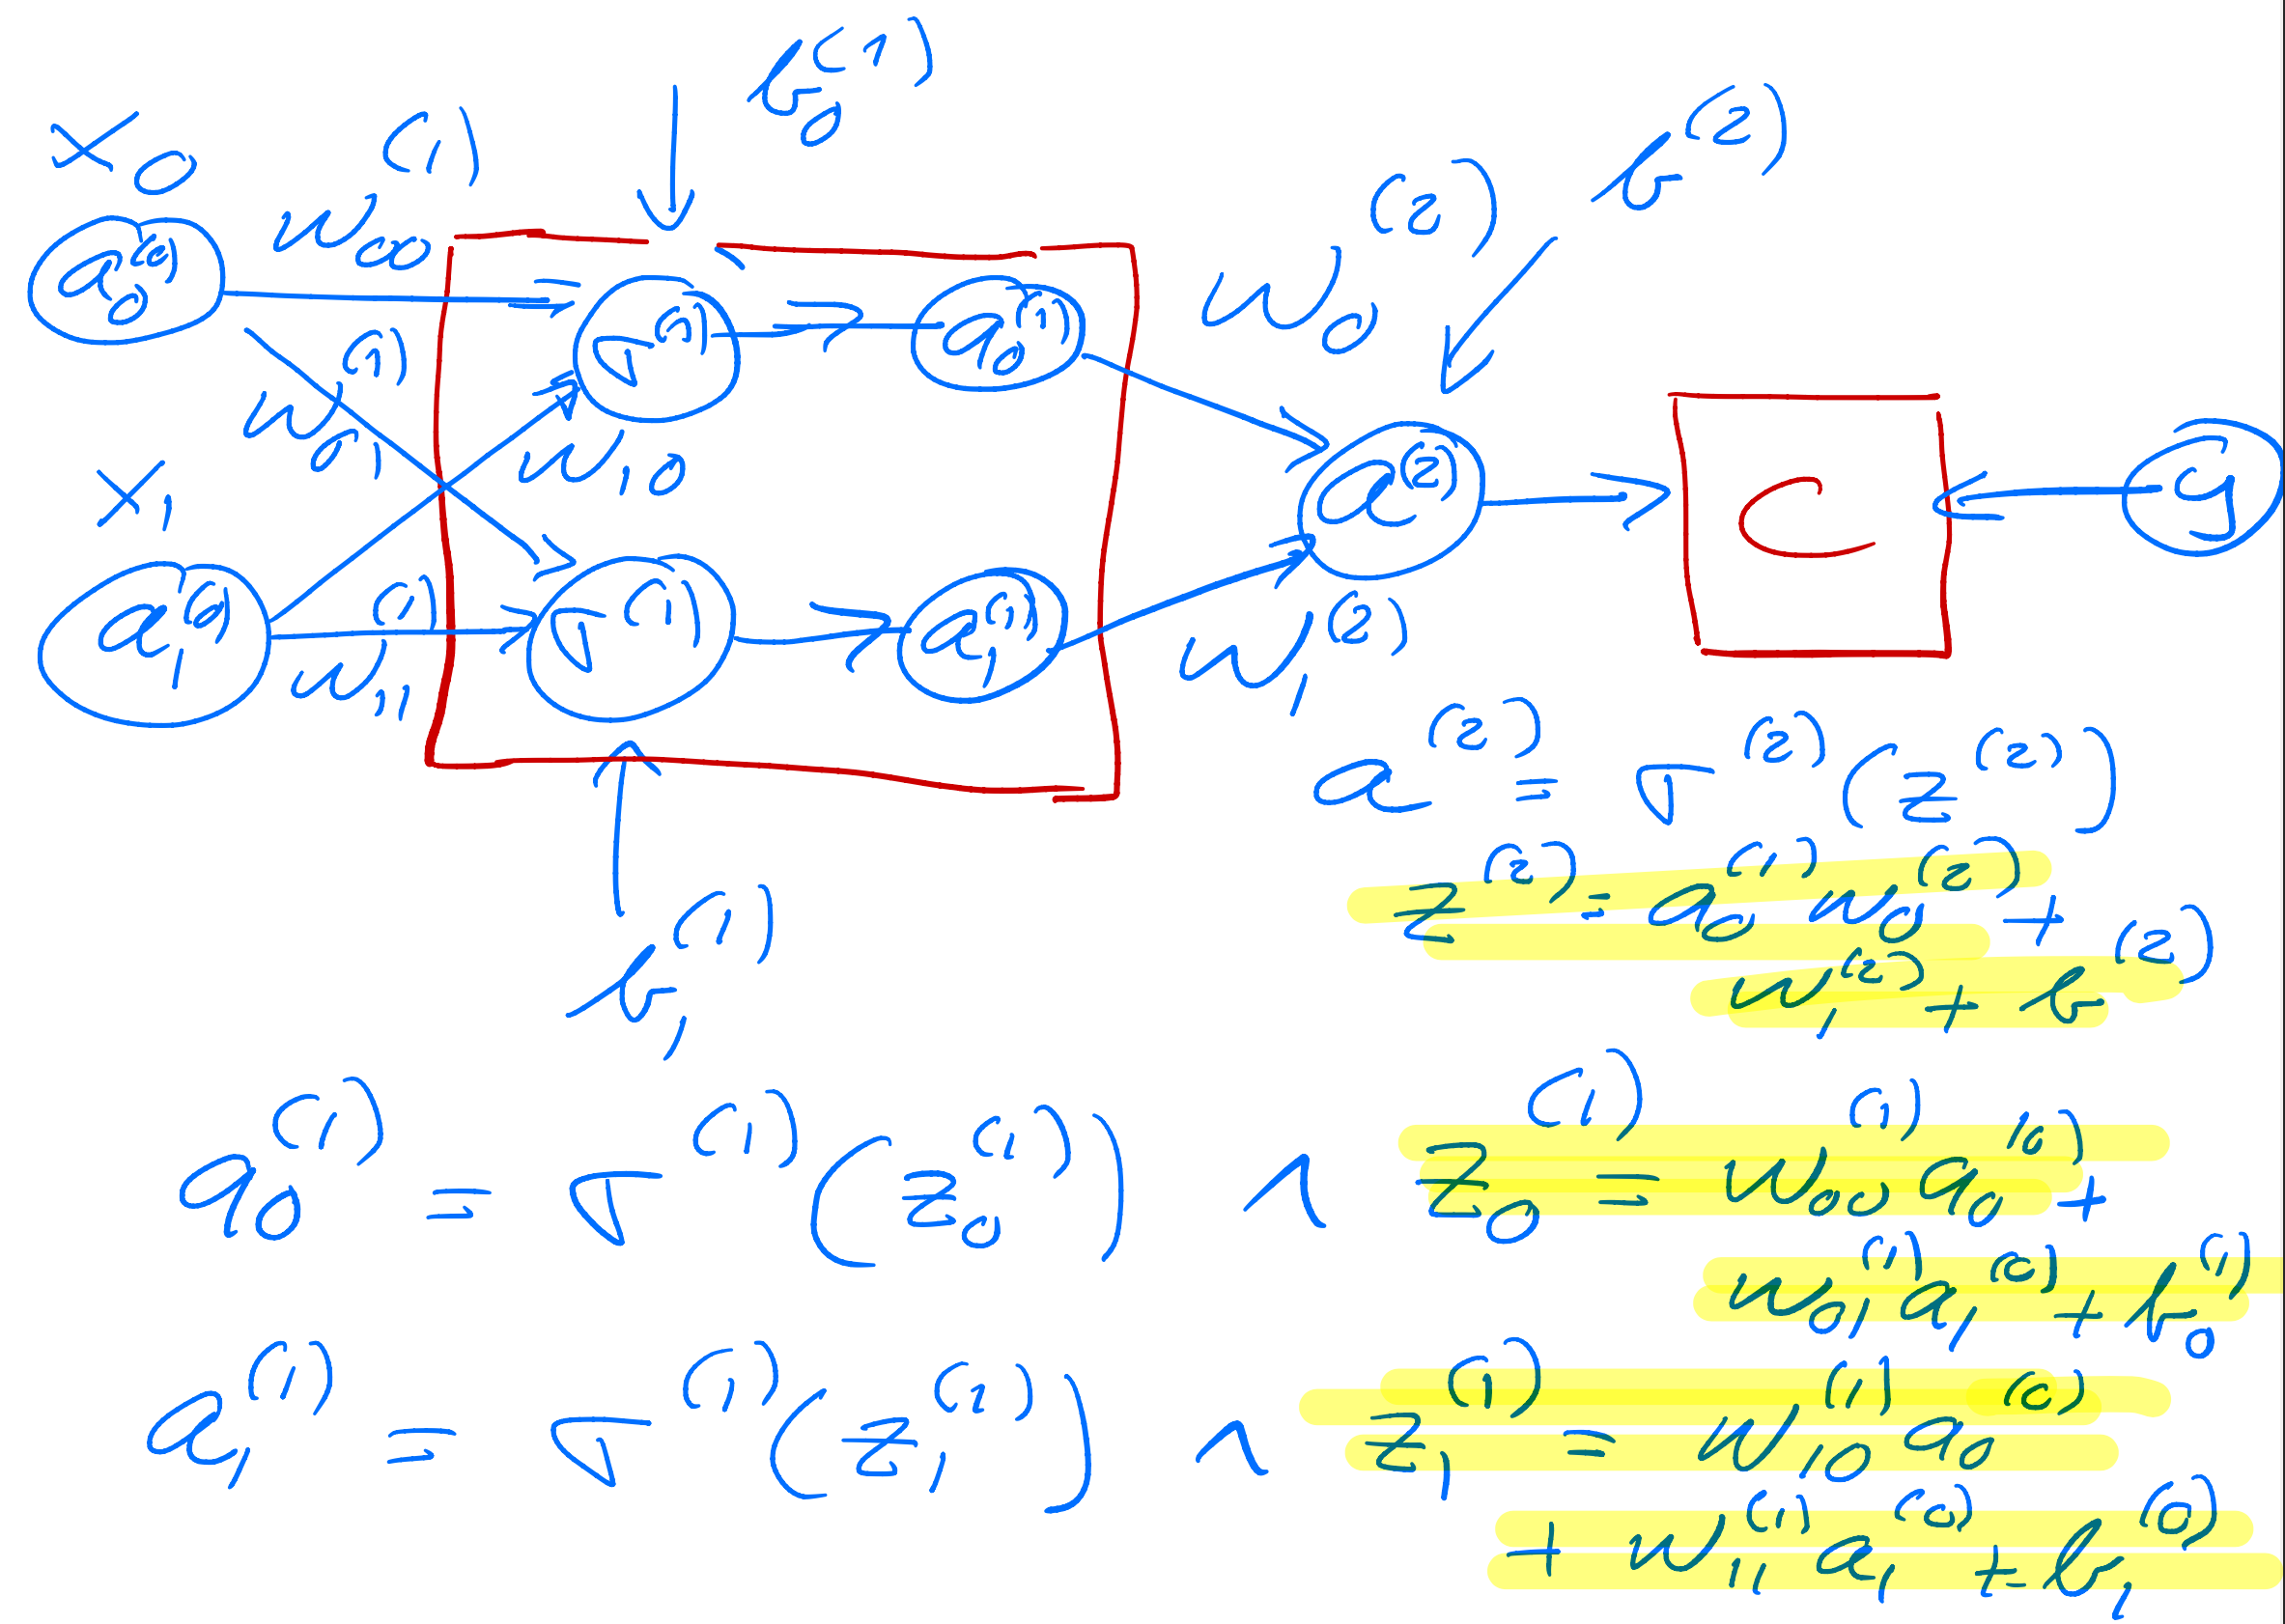
\includegraphics[width=1.0\linewidth]{figures/simplenn3.png}}

\vspace{6mm}
\end{frame}

\begin{frame}[plain,fragile]
\frametitle{The ouput layer}

Finally, we have the ouput layer given by layer label $(2)$ with output $a^{(2)}$ and weights and biases to be determined given by the variables
\[
w_{i}^{(2)}=\left\{w_{0}^{(2)},w_{1}^{(2)}\right\} \wedge b^{(2)}.
\]

Our output is $\tilde{y}=a^{(2)}$ and we define a generic cost function $C(a^{(2)},y;\bm{\Theta})$ where $y$ is the target value (a scalar here).
The parameters we need to optimize are given by
\[
\bm{\Theta}=\left\{w_{00}^{(1)},w_{01}^{(1)},w_{10}^{(1)},w_{11}^{(1)},w_{0}^{(2)},w_{1}^{(2)},b_0^{(1)},b_1^{(1)},b^{(2)}\right\}.
\]
\end{frame}

\begin{frame}[plain,fragile]
\frametitle{Compact expressions}

We can define the inputs to the activation functions for the various layers in terms of various matrix-vector multiplications and vector additions.
The inputs to the first hidden layer are
\[
\begin{bmatrix}z_0^{(1)} \\ z_1^{(1)} \end{bmatrix}=\begin{bmatrix}w_{00}^{(1)} & w_{01}^{(1)}\\ w_{10}^{(1)} &w_{11}^{(1)} \end{bmatrix}\begin{bmatrix}a_0^{(0)} \\ a_1^{(0)} \end{bmatrix}+\begin{bmatrix}b_0^{(1)} \\ b_1^{(1)} \end{bmatrix},
\]
with outputs
\[
\begin{bmatrix}a_0^{(1)} \\ a_1^{(1)} \end{bmatrix}=\begin{bmatrix}\sigma^{(1)}(z_0^{(1)}) \\ \sigma^{(1)}(z_1^{(1)}) \end{bmatrix}.
\]
\end{frame}

\begin{frame}[plain,fragile]
\frametitle{Output layer}

For the final output layer we have the inputs to the final activation function 
\[
z^{(2)} = w_{0}^{(2)}a_0^{(1)} +w_{1}^{(2)}a_1^{(1)}+b^{(2)},
\]
resulting in the  output
\[
a^{(2)}=\sigma^{(2)}(z^{(2)}).
\]
\end{frame}

\begin{frame}[plain,fragile]
\frametitle{Explicit derivatives}

In total we have nine parameters which we need to train.  Using the
chain rule (or just the back-propagation algorithm) we can find all
derivatives. Since we will use automatic differentiation in reverse
mode, we start with the derivatives of the cost function with respect
to the parameters of the output layer, namely

\[
\frac{\partial C}{\partial w_{i}^{(2)}}=\frac{\partial C}{\partial a^{(2)}}\frac{\partial a^{(2)}}{\partial z^{(2)}}\frac{\partial z^{(2)}}{\partial w_{i}^{(2)}}=\delta^{(2)}a_i^{(1)},
\]
with
\[
\delta^{(2)}=\frac{\partial C}{\partial a^{(2)}}\frac{\partial a^{(2)}}{\partial z^{(2)}}
\]
and finally
\[
\frac{\partial C}{\partial b^{(2)}}=\frac{\partial C}{\partial a^{(2)}}\frac{\partial a^{(2)}}{\partial z^{(2)}}\frac{\partial z^{(2)}}{\partial b^{(2)}}=\delta^{(2)}.
\]
\end{frame}

\begin{frame}[plain,fragile]
\frametitle{Derivatives of the hidden layer}

Using the chain rule we have the following expressions for say one of the weight parameters (it is easy to generalize to the other weight parameters)
\[
\frac{\partial C}{\partial w_{00}^{(1)}}=\frac{\partial C}{\partial a^{(2)}}\frac{\partial a^{(2)}}{\partial z^{(2)}}
\frac{\partial z^{(2)}}{\partial z_0^{(1)}}\frac{\partial z_0^{(1)}}{\partial w_{00}^{(1)}}=    \delta^{(2)}\frac{\partial z^{(2)}}{\partial z_0^{(1)}}\frac{\partial z_0^{(1)}}{\partial w_{00}^{(1)}},
\]
which, noting that
\[
z^{(2)} =w_0^{(2)}a_0^{(1)}+w_1^{(2)}a_1^{(1)}+b^{(2)},
\]
allows us to rewrite 
\[
\frac{\partial z^{(2)}}{\partial z_0^{(1)}}\frac{\partial z_0^{(1)}}{\partial w_{00}^{(1)}}=w_0^{(2)}\frac{\partial a_0^{(1)}}{\partial z_0^{(1)}}a_0^{(1)}.
\]
\end{frame}

\begin{frame}[plain,fragile]
\frametitle{Final expression}

Defining
\[
\delta_0^{(1)}=w_0^{(2)}\frac{\partial a_0^{(1)}}{\partial z_0^{(1)}}\delta^{(2)},
\]
we have 
\[
\frac{\partial C}{\partial w_{00}^{(1)}}=\delta_0^{(1)}a_0^{(1)}.
\]
Similarly, we obtain
\[
\frac{\partial C}{\partial w_{01}^{(1)}}=\delta_0^{(1)}a_1^{(1)}.
\]
\end{frame}

\begin{frame}[plain,fragile]
\frametitle{Completing the list}

Similarly, we find
\[
\frac{\partial C}{\partial w_{10}^{(1)}}=\delta_1^{(1)}a_0^{(1)},
\]
and 
\[
\frac{\partial C}{\partial w_{11}^{(1)}}=\delta_1^{(1)}a_1^{(1)},
\]
where we have defined 
\[
\delta_1^{(1)}=w_1^{(2)}\frac{\partial a_1^{(1)}}{\partial z_1^{(1)}}\delta^{(2)}.
\]
\end{frame}

\begin{frame}[plain,fragile]
\frametitle{Final expressions for the biases of the hidden layer}

For the sake of completeness, we list the derivatives of the biases, which are
\[
\frac{\partial C}{\partial b_{0}^{(1)}}=\delta_0^{(1)},
\]
and
\[
\frac{\partial C}{\partial b_{1}^{(1)}}=\delta_1^{(1)}.
\]
As we will see below, these expressions can be generalized in a more compact form.
\end{frame}

\begin{frame}[plain,fragile]
\frametitle{Gradient expressions}

For this specific model, with just one output node and two hidden
nodes, the gradient descent equations take the following form for output layer
\[
w_{i}^{(2)}\leftarrow w_{i}^{(2)}- \eta \delta^{(2)} a_{i}^{(1)},
\]
and
\[
b^{(2)} \leftarrow b^{(2)}-\eta \delta^{(2)},
\]
and
\[
w_{ij}^{(1)}\leftarrow w_{ij}^{(1)}- \eta \delta_{i}^{(1)} a_{j}^{(0)},
\]
and
\[
b_{i}^{(1)} \leftarrow b_{i}^{(1)}-\eta \delta_{i}^{(1)},
\]
where $\eta$ is the learning rate.
\end{frame}

\begin{frame}[plain,fragile]
% No title on this slide

% --- begin exercise ---
\begin{doconceexercise}
\refstepcounter{doconceexercisecounter}

\exercisesection{Exercise \thedoconceexercisecounter: Extended program}
                             

We extend our simple code to a function which depends on two variable $x_0$ and $x_1$, that is
\[
y=f(x_0,x_1)=x_0^2+3x_0x_1+x_1^2+5.
\]
We feed our network with $n=100$ entries $x_0$ and $x_1$. We have thus two features represented by these variable and an input matrix/design matrix $\bm{X}\in \mathbf{R}^{n\times 2}$
\[
\bm{X}=\begin{bmatrix} x_{00} & x_{01} \\ x_{00} & x_{01} \\ x_{10} & x_{11} \\ x_{20} & x_{21} \\ \dots & \dots \\ \dots & \dots \\ x_{n-20} & x_{n-21} \\ x_{n-10} & x_{n-11} \end{bmatrix}.
\]
Write a code, based on the previous code examples, which takes as input these data and fit the above function.
You can extend your code to include automatic differentiation.

With these examples, we are now ready to embark upon the writing of more a general code for neural networks.

\end{doconceexercise}
% --- end exercise ---
\end{frame}

\begin{frame}[plain,fragile]
\frametitle{Getting serious, the  back propagation equations for a neural network}

Now it is time to move away from one node in each layer only. Our inputs are also represented either by several inputs.

We have thus
\[
\frac{\partial{\cal C}((\bm{\Theta}^L)}{\partial w_{jk}^L}  =  \left(a_j^L - y_j\right)a_j^L(1-a_j^L)a_k^{L-1}, 
\]

Defining
\[
\delta_j^L = a_j^L(1-a_j^L)\left(a_j^L - y_j\right) = \sigma'(z_j^L)\frac{\partial {\cal C}}{\partial (a_j^L)},
\]
and using the Hadamard product of two vectors we can write this as
\[
\bm{\delta}^L = \sigma'(\hat{z}^L)\circ\frac{\partial {\cal C}}{\partial (\bm{a}^L)}.
\]
\end{frame}

\begin{frame}[plain,fragile]
\frametitle{Analyzing the last results}

This is an important expression. The second term on the right handside
measures how fast the cost function is changing as a function of the $j$th
output activation.  If, for example, the cost function doesn't depend
much on a particular output node $j$, then $\delta_j^L$ will be small,
which is what we would expect. The first term on the right, measures
how fast the activation function $f$ is changing at a given activation
value $z_j^L$.
\end{frame}

\begin{frame}[plain,fragile]
\frametitle{More considerations}

Notice that everything in the above equations is easily computed.  In
particular, we compute $z_j^L$ while computing the behaviour of the
network, and it is only a small additional overhead to compute
$\sigma'(z^L_j)$.  The exact form of the derivative with respect to the
output depends on the form of the cost function.
However, provided the cost function is known there should be little
trouble in calculating

\[
\frac{\partial {\cal C}}{\partial (a_j^L)}
\]

With the definition of $\delta_j^L$ we have a more compact definition of the derivative of the cost function in terms of the weights, namely
\[
\frac{\partial{\cal C}}{\partial w_{jk}^L}  =  \delta_j^La_k^{L-1}.
\]
\end{frame}

\begin{frame}[plain,fragile]
\frametitle{Derivatives in terms of $z_j^L$}

It is also easy to see that our previous equation can be written as

\[
\delta_j^L =\frac{\partial {\cal C}}{\partial z_j^L}= \frac{\partial {\cal C}}{\partial a_j^L}\frac{\partial a_j^L}{\partial z_j^L},
\]
which can also be interpreted as the partial derivative of the cost function with respect to the biases $b_j^L$, namely
\[
\delta_j^L = \frac{\partial {\cal C}}{\partial b_j^L}\frac{\partial b_j^L}{\partial z_j^L}=\frac{\partial {\cal C}}{\partial b_j^L},
\]
That is, the error $\delta_j^L$ is exactly equal to the rate of change of the cost function as a function of the bias.
\end{frame}

\begin{frame}[plain,fragile]
\frametitle{Bringing it together}

We have now three equations that are essential for the computations of the derivatives of the cost function at the output layer. These equations are needed to start the algorithm and they are

\begin{equation}
\frac{\partial{\cal C}(\hat{W^L})}{\partial w_{jk}^L}  =  \delta_j^La_k^{L-1},
\end{equation}
and
\begin{equation}
\delta_j^L = \sigma'(z_j^L)\frac{\partial {\cal C}}{\partial (a_j^L)},
\end{equation}
and

\begin{equation}
\delta_j^L = \frac{\partial {\cal C}}{\partial b_j^L},
\end{equation}
\end{frame}

\begin{frame}[plain,fragile]
\frametitle{Final back propagating equation}

We have that (replacing $L$ with a general layer $l$)
\[
\delta_j^l =\frac{\partial {\cal C}}{\partial z_j^l}.
\]
We want to express this in terms of the equations for layer $l+1$.
\end{frame}

\begin{frame}[plain,fragile]
\frametitle{Using the chain rule and summing over all $k$ entries}

We obtain
\[
\delta_j^l =\sum_k \frac{\partial {\cal C}}{\partial z_k^{l+1}}\frac{\partial z_k^{l+1}}{\partial z_j^{l}}=\sum_k \delta_k^{l+1}\frac{\partial z_k^{l+1}}{\partial z_j^{l}},
\]
and recalling that
\[
z_j^{l+1} = \sum_{i=1}^{M_{l}}w_{ij}^{l+1}a_i^{l}+b_j^{l+1},
\]
with $M_l$ being the number of nodes in layer $l$, we obtain
\[
\delta_j^l =\sum_k \delta_k^{l+1}w_{kj}^{l+1}\sigma'(z_j^l),
\]
This is our final equation.

We are now ready to set up the algorithm for back propagation and learning the weights and biases.
\end{frame}

\begin{frame}[plain,fragile]
\frametitle{Setting up the back propagation algorithm}

The four equations  provide us with a way of computing the gradient of the cost function. Let us write this out in the form of an algorithm.

\textbf{First}, we set up the input data $\hat{x}$ and the activations
$\hat{z}_1$ of the input layer and compute the activation function and
the pertinent outputs $\hat{a}^1$.

\textbf{Secondly}, we perform then the feed forward till we reach the output
layer and compute all $\hat{z}_l$ of the input layer and compute the
activation function and the pertinent outputs $\hat{a}^l$ for
$l=1,2,3,\dots,L$.

\textbf{Notation}: The first hidden layer has $l=1$ as label and the final output layer has $l=L$.
\end{frame}

\begin{frame}[plain,fragile]
\frametitle{Setting up the back propagation algorithm, part 2}

Thereafter we compute the ouput error $\hat{\delta}^L$ by computing all
\[
\delta_j^L = \sigma'(z_j^L)\frac{\partial {\cal C}}{\partial (a_j^L)}.
\]

Then we compute the back propagate error for each $l=L-1,L-2,\dots,1$ as
\[
\delta_j^l = \sum_k \delta_k^{l+1}w_{kj}^{l+1}\sigma'(z_j^l).
\]
\end{frame}

\begin{frame}[plain,fragile]
\frametitle{Setting up the Back propagation algorithm, part 3}

Finally, we update the weights and the biases using gradient descent
for each $l=L-1,L-2,\dots,1$ and update the weights and biases
according to the rules

\[
w_{jk}^l\leftarrow  = w_{jk}^l- \eta \delta_j^la_k^{l-1},
\]

\[
b_j^l \leftarrow b_j^l-\eta \frac{\partial {\cal C}}{\partial b_j^l}=b_j^l-\eta \delta_j^l,
\]
with $\eta$ being the learning rate.
\end{frame}

\begin{frame}[plain,fragile]
\frametitle{Updating the gradients}

With the back propagate error for each $l=L-1,L-2,\dots,1$ as
\[
\delta_j^l = \sum_k \delta_k^{l+1}w_{kj}^{l+1}sigma'(z_j^l),
\]
we update the weights and the biases using gradient descent for each $l=L-1,L-2,\dots,1$ and update the weights and biases according to the rules
\[
w_{jk}^l\leftarrow  = w_{jk}^l- \eta \delta_j^la_k^{l-1},
\]

\[
b_j^l \leftarrow b_j^l-\eta \frac{\partial {\cal C}}{\partial b_j^l}=b_j^l-\eta \delta_j^l,
\]
\end{frame}

\begin{frame}[plain,fragile]
% No title on this slide

\noindent\textbf{Activation functions.}
A property that characterizes a neural network, other than its
connectivity, is the choice of activation function(s).  As described
in, the following restrictions are imposed on an activation function
for a FFNN to fulfill the universal approximation theorem

\begin{itemize}
  \item Non-constant

  \item Bounded

  \item Monotonically-increasing

  \item Continuous
\end{itemize}

\noindent
\end{frame}

\begin{frame}[plain,fragile]
% No title on this slide

\noindent\textbf{Activation functions, Logistic and Hyperbolic ones.}
The second requirement excludes all linear functions. Furthermore, in
a MLP with only linear activation functions, each layer simply
performs a linear transformation of its inputs.

Regardless of the number of layers, the output of the NN will be
nothing but a linear function of the inputs. Thus we need to introduce
some kind of non-linearity to the NN to be able to fit non-linear
functions Typical examples are the logistic \emph{Sigmoid}

\[
 f(x) = \frac{1}{1 + e^{-x}},
\]
and the \emph{hyperbolic tangent} function
\[
 f(x) = \tanh(x)
\]
\end{frame}

\begin{frame}[plain,fragile]
% No title on this slide

\noindent\textbf{Relevance.}
The \emph{sigmoid} function are more biologically plausible because the
output of inactive neurons are zero. Such activation function are
called \emph{one-sided}. However, it has been shown that the hyperbolic
tangent performs better than the sigmoid for training MLPs.  has
become the most popular for \emph{deep neural networks}









































































\begin{minted}[fontsize=\fontsize{9pt}{9pt},linenos=false,mathescape,baselinestretch=1.0,fontfamily=tt,xleftmargin=2mm]{python}
"""The sigmoid function (or the logistic curve) is a 
function that takes any real number, z, and outputs a number (0,1).
It is useful in neural networks for assigning weights on a relative scale.
The value z is the weighted sum of parameters involved in the learning algorithm."""

import numpy
import matplotlib.pyplot as plt
import math as mt

z = numpy.arange(-5, 5, .1)
sigma_fn = numpy.vectorize(lambda z: 1/(1+numpy.exp(-z)))
sigma = sigma_fn(z)

fig = plt.figure()
ax = fig.add_subplot(111)
ax.plot(z, sigma)
ax.set_ylim([-0.1, 1.1])
ax.set_xlim([-5,5])
ax.grid(True)
ax.set_xlabel('z')
ax.set_title('sigmoid function')

plt.show()

"""Step Function"""
z = numpy.arange(-5, 5, .02)
step_fn = numpy.vectorize(lambda z: 1.0 if z >= 0.0 else 0.0)
step = step_fn(z)

fig = plt.figure()
ax = fig.add_subplot(111)
ax.plot(z, step)
ax.set_ylim([-0.5, 1.5])
ax.set_xlim([-5,5])
ax.grid(True)
ax.set_xlabel('z')
ax.set_title('step function')

plt.show()

"""Sine Function"""
z = numpy.arange(-2*mt.pi, 2*mt.pi, 0.1)
t = numpy.sin(z)

fig = plt.figure()
ax = fig.add_subplot(111)
ax.plot(z, t)
ax.set_ylim([-1.0, 1.0])
ax.set_xlim([-2*mt.pi,2*mt.pi])
ax.grid(True)
ax.set_xlabel('z')
ax.set_title('sine function')

plt.show()

"""Plots a graph of the squashing function used by a rectified linear
unit"""
z = numpy.arange(-2, 2, .1)
zero = numpy.zeros(len(z))
y = numpy.max([zero, z], axis=0)

fig = plt.figure()
ax = fig.add_subplot(111)
ax.plot(z, y)
ax.set_ylim([-2.0, 2.0])
ax.set_xlim([-2.0, 2.0])
ax.grid(True)
ax.set_xlabel('z')
ax.set_title('Rectified linear unit')

plt.show()

\end{minted}
\end{frame}

\begin{frame}[plain,fragile]
\frametitle{Fine-tuning neural network hyperparameters}

The flexibility of neural networks is also one of their main
drawbacks: there are many hyperparameters to tweak. Not only can you
use any imaginable network topology (how neurons/nodes are
interconnected), but even in a simple FFNN you can change the number
of layers, the number of neurons per layer, the type of activation
function to use in each layer, the weight initialization logic, the
stochastic gradient optmized and much more. How do you know what
combination of hyperparameters is the best for your task?

\begin{itemize}
\item You can use grid search with cross-validation to find the right hyperparameters.
\end{itemize}

\noindent
However,since there are many hyperparameters to tune, and since
training a neural network on a large dataset takes a lot of time, you
will only be able to explore a tiny part of the hyperparameter space.

\begin{itemize}
\item You can use randomized search.

\item Or use tools like \href{{http://oscar.calldesk.ai/}}{Oscar}, which implements more complex algorithms to help you find a good set of hyperparameters quickly.  
\end{itemize}

\noindent
\end{frame}

\begin{frame}[plain,fragile]
\frametitle{Hidden layers}

For many problems you can start with just one or two hidden layers and
it will work just fine.  For the MNIST data set you ca easily get a
high accuracy using just one hidden layer with a few hundred neurons.
You can reach for this data set above 98\% accuracy using two hidden
layers with the same total amount of neurons, in roughly the same
amount of training time.

For more complex problems, you can gradually ramp up the number of
hidden layers, until you start overfitting the training set. Very
complex tasks, such as large image classification or speech
recognition, typically require networks with dozens of layers and they
need a huge amount of training data. However, you will rarely have to
train such networks from scratch: it is much more common to reuse
parts of a pretrained state-of-the-art network that performs a similar
task.
\end{frame}

\begin{frame}[plain,fragile]
\frametitle{Vanishing gradients}

The Back propagation algorithm we derived above works by going from
the output layer to the input layer, propagating the error gradient on
the way. Once the algorithm has computed the gradient of the cost
function with regards to each parameter in the network, it uses these
gradients to update each parameter with a Gradient Descent (GD) step.

Unfortunately for us, the gradients often get smaller and smaller as
the algorithm progresses down to the first hidden layers. As a result,
the GD update leaves the lower layer connection weights virtually
unchanged, and training never converges to a good solution. This is
known in the literature as \textbf{the vanishing gradients problem}.
\end{frame}

\begin{frame}[plain,fragile]
\frametitle{Exploding gradients}

In other cases, the opposite can happen, namely the the gradients can
grow bigger and bigger. The result is that many of the layers get
large updates of the weights the algorithm diverges. This is the
\textbf{exploding gradients problem}, which is mostly encountered in
recurrent neural networks. More generally, deep neural networks suffer
from unstable gradients, different layers may learn at widely
different speeds
\end{frame}

\begin{frame}[plain,fragile]
\frametitle{Is the Logistic activation function (Sigmoid)  our choice?}

Although this unfortunate behavior has been empirically observed for
quite a while (it was one of the reasons why deep neural networks were
mostly abandoned for a long time), it is only around 2010 that
significant progress was made in understanding it.

A paper titled \href{{http://proceedings.mlr.press/v9/glorot10a.html}}{Understanding the Difficulty of Training Deep
Feedforward Neural Networks by Xavier Glorot and Yoshua Bengio} found that
the problems with the popular logistic
sigmoid activation function and the weight initialization technique
that was most popular at the time, namely random initialization using
a normal distribution with a mean of 0 and a standard deviation of
1.
\end{frame}

\begin{frame}[plain,fragile]
\frametitle{Logistic function as the root of problems}

They showed that with this activation function and this
initialization scheme, the variance of the outputs of each layer is
much greater than the variance of its inputs. Going forward in the
network, the variance keeps increasing after each layer until the
activation function saturates at the top layers. This is actually made
worse by the fact that the logistic function has a mean of 0.5, not 0
(the hyperbolic tangent function has a mean of 0 and behaves slightly
better than the logistic function in deep networks).
\end{frame}

\begin{frame}[plain,fragile]
\frametitle{The derivative of the Logistic funtion}

Looking at the logistic activation function, when inputs become large
(negative or positive), the function saturates at 0 or 1, with a
derivative extremely close to 0. Thus when backpropagation kicks in,
it has virtually no gradient to propagate back through the network,
and what little gradient exists keeps getting diluted as
backpropagation progresses down through the top layers, so there is
really nothing left for the lower layers.

In their paper, Glorot and Bengio propose a way to significantly
alleviate this problem. We need the signal to flow properly in both
directions: in the forward direction when making predictions, and in
the reverse direction when backpropagating gradients. We don’t want
the signal to die out, nor do we want it to explode and saturate. For
the signal to flow properly, the authors argue that we need the
variance of the outputs of each layer to be equal to the variance of
its inputs, and we also need the gradients to have equal variance
before and after flowing through a layer in the reverse direction.
\end{frame}

\begin{frame}[plain,fragile]
\frametitle{Insights from the paper by Glorot and Bengio}

One of the insights in the 2010 paper by Glorot and Bengio was that
the vanishing/exploding gradients problems were in part due to a poor
choice of activation function. Until then most people had assumed that
if Nature had chosen to use roughly sigmoid activation functions in
biological neurons, they must be an excellent choice. But it turns out
that other activation functions behave much better in deep neural
networks, in particular the ReLU activation function, mostly because
it does not saturate for positive values (and also because it is quite
fast to compute).
\end{frame}

\begin{frame}[plain,fragile]
\frametitle{The RELU function family}

The ReLU activation function suffers from a problem known as the dying
ReLUs: during training, some neurons effectively die, meaning they
stop outputting anything other than 0.

In some cases, you may find that half of your network’s neurons are
dead, especially if you used a large learning rate. During training,
if a neuron’s weights get updated such that the weighted sum of the
neuron’s inputs is negative, it will start outputting 0. When this
happen, the neuron is unlikely to come back to life since the gradient
of the ReLU function is 0 when its input is negative.
\end{frame}

\begin{frame}[plain,fragile]
\frametitle{ELU function}

To solve this problem, nowadays practitioners use a variant of the
ReLU function, such as the leaky ReLU discussed above or the so-called
exponential linear unit (ELU) function

\[
ELU(z) = \left\{\begin{array}{cc} \alpha\left( \exp{(z)}-1\right) & z < 0,\\  z & z \ge 0.\end{array}\right. 
\]
\end{frame}

\begin{frame}[plain,fragile]
\frametitle{Which activation function should we use?}

In general it seems that the ELU activation function is better than
the leaky ReLU function (and its variants), which is better than
ReLU. ReLU performs better than $\tanh$ which in turn performs better
than the logistic function.

If runtime performance is an issue, then you may opt for the leaky
ReLU function over the ELU function If you don’t want to tweak yet
another hyperparameter, you may just use the default $\alpha$ of
$0.01$ for the leaky ReLU, and $1$ for ELU. If you have spare time and
computing power, you can use cross-validation or bootstrap to evaluate
other activation functions.
\end{frame}

\begin{frame}[plain,fragile]
\frametitle{More on activation functions, output layers}

In most cases you can use the ReLU activation function in the hidden
layers (or one of its variants).

It is a bit faster to compute than other activation functions, and the
gradient descent optimization does in general not get stuck.

\textbf{For the output layer:}

\begin{itemize}
\item For classification the softmax activation function is generally a good choice for classification tasks (when the classes are mutually exclusive).

\item For regression tasks, you can simply use no activation function at all.
\end{itemize}

\noindent
\end{frame}

\begin{frame}[plain,fragile]
\frametitle{Batch Normalization}

Batch Normalization aims to address the vanishing/exploding gradients
problems, and more generally the problem that the distribution of each
layer’s inputs changes during training, as the parameters of the
previous layers change.

The technique consists of adding an operation in the model just before
the activation function of each layer, simply zero-centering and
normalizing the inputs, then scaling and shifting the result using two
new parameters per layer (one for scaling, the other for shifting). In
other words, this operation lets the model learn the optimal scale and
mean of the inputs for each layer.  In order to zero-center and
normalize the inputs, the algorithm needs to estimate the inputs’ mean
and standard deviation. It does so by evaluating the mean and standard
deviation of the inputs over the current mini-batch, from this the
name batch normalization.
\end{frame}

\begin{frame}[plain,fragile]
\frametitle{Dropout}

It is a fairly simple algorithm: at every training step, every neuron
(including the input neurons but excluding the output neurons) has a
probability $p$ of being temporarily dropped out, meaning it will be
entirely ignored during this training step, but it may be active
during the next step.

The hyperparameter $p$ is called the dropout rate, and it is typically
set to 50\%. After training, the neurons are not dropped anymore.  It
is viewed as one of the most popular regularization techniques.
\end{frame}

\begin{frame}[plain,fragile]
\frametitle{Gradient Clipping}

A popular technique to lessen the exploding gradients problem is to
simply clip the gradients during backpropagation so that they never
exceed some threshold (this is mostly useful for recurrent neural
networks).

This technique is called Gradient Clipping.

In general however, Batch
Normalization is preferred.
\end{frame}

\begin{frame}[plain,fragile]
\frametitle{A top-down perspective on Neural networks}

The first thing we would like to do is divide the data into two or
three parts. A training set, a validation or dev (development) set,
and a test set. The test set is the data on which we want to make
predictions. The dev set is a subset of the training data we use to
check how well we are doing out-of-sample, after training the model on
the training dataset. We use the validation error as a proxy for the
test error in order to make tweaks to our model. It is crucial that we
do not use any of the test data to train the algorithm. This is a
cardinal sin in ML. Then:

\begin{enumerate}
\item Estimate optimal error rate

\item Minimize underfitting (bias) on training data set.

\item Make sure you are not overfitting.
\end{enumerate}

\noindent
\end{frame}

\begin{frame}[plain,fragile]
\frametitle{More top-down perspectives}

If the validation and test sets are drawn from the same distributions,
then a good performance on the validation set should lead to similarly
good performance on the test set. 

However, sometimes
the training data and test data differ in subtle ways because, for
example, they are collected using slightly different methods, or
because it is cheaper to collect data in one way versus another. In
this case, there can be a mismatch between the training and test
data. This can lead to the neural network overfitting these small
differences between the test and training sets, and a poor performance
on the test set despite having a good performance on the validation
set. To rectify this, Andrew Ng suggests making two validation or dev
sets, one constructed from the training data and one constructed from
the test data. The difference between the performance of the algorithm
on these two validation sets quantifies the train-test mismatch. This
can serve as another important diagnostic when using DNNs for
supervised learning.
\end{frame}

\begin{frame}[plain,fragile]
\frametitle{Limitations of supervised learning with deep networks}

Like all statistical methods, supervised learning using neural
networks has important limitations. This is especially important when
one seeks to apply these methods, especially to physics problems. Like
all tools, DNNs are not a universal solution. Often, the same or
better performance on a task can be achieved by using a few
hand-engineered features (or even a collection of random
features).
\end{frame}

\begin{frame}[plain,fragile]
\frametitle{Limitations of NNs}

Here we list some of the important limitations of supervised neural network based models. 

\begin{itemize}
\item \textbf{Need labeled data}. All supervised learning methods, DNNs for supervised learning require labeled data. Often, labeled data is harder to acquire than unlabeled data (e.g.~one must pay for human experts to label images).

\item \textbf{Supervised neural networks are extremely data intensive.} DNNs are data hungry. They perform best when data is plentiful. This is doubly so for supervised methods where the data must also be labeled. The utility of DNNs is extremely limited if data is hard to acquire or the datasets are small (hundreds to a few thousand samples). In this case, the performance of other methods that utilize hand-engineered features can exceed that of DNNs.
\end{itemize}

\noindent
\end{frame}

\begin{frame}[plain,fragile]
\frametitle{Homogeneous data}

\begin{itemize}
\item \textbf{Homogeneous data.} Almost all DNNs deal with homogeneous data of one type. It is very hard to design architectures that mix and match data types (i.e.~some continuous variables, some discrete variables, some time series). In applications beyond images, video, and language, this is often what is required. In contrast, ensemble models like random forests or gradient-boosted trees have no difficulty handling mixed data types.
\end{itemize}

\noindent
\end{frame}

\begin{frame}[plain,fragile]
\frametitle{More limitations}

\begin{itemize}
\item \textbf{Many problems are not about prediction.} In natural science we are often interested in learning something about the underlying distribution that generates the data. In this case, it is often difficult to cast these ideas in a supervised learning setting. While the problems are related, it is possible to make good predictions with a \emph{wrong} model. The model might or might not be useful for understanding the underlying science.
\end{itemize}

\noindent
Some of these remarks are particular to DNNs, others are shared by all supervised learning methods. This motivates the use of unsupervised methods which in part circumvent these problems.
\end{frame}

\end{document}
